\documentclass[a4paper]{report}
\usepackage[utf8]{inputenc}
\usepackage{hyperref}
\usepackage{natbib} % Bibliography package
%\bibliographystyle{ksfh_nat}
\usepackage{graphicx}
\usepackage[english]{babel}
\usepackage{enumitem}
\usepackage{listings}
\usepackage{filecontents}
\usepackage{verbatim}
\usepackage{eurosym}
\usepackage[export]{adjustbox}
\usepackage{titlesec}
\usepackage[utf8]{inputenc}
\usepackage[english]{babel}
%\usepackage[T1, T2A]{fontenc}
\usepackage{amsmath}
\usepackage{mdframed}
\usepackage{pdfpages}

\usepackage{etoolbox,refcount}
\usepackage{multicol}

\usepackage{booktabs}
\usepackage{tabularx}
\usepackage{lipsum}

\usepackage{listings} % code highlighting
\usepackage{tikz} % drawing
\usepackage{commath} % \norm

\usepackage{dirtree}
\usepackage{float}

\usepackage{isodate}

\usepackage[style=ieee, citestyle=numeric, sorting=none]{biblatex}
\addbibresource{bibliography/bibliography.bib}          % papers
\addbibresource{bibliography/otherimplementations.bib}  % hrefs to examples of other implementations

\usepackage[toc,page]{appendix}


\titleformat{\chapter}[display]
  {\bfseries\huge}
  {\bigskip\filleft\Large\chaptertitlename~\thechapter}
  {3ex}
  {\titlerule\vspace{1.5ex}\filright}
  [\vspace{1ex}\titlerule]



\usepackage{afterpage}

\newcommand\blankpage{%
    \null
    \thispagestyle{empty}%
    \addtocounter{page}{-1}%
    \newpage}






% =============================== ITEMIZE COLUMNS =================================================================%

\newcounter{countitems}
\newcounter{nextitemizecount}
\newcommand{\setupcountitems}{%
  \stepcounter{nextitemizecount}%
  \setcounter{countitems}{0}%
  \preto\item{\stepcounter{countitems}}%
}
\makeatletter
\newcommand{\computecountitems}{%
  \edef\@currentlabel{\number\c@countitems}%
  \label{countitems@\number\numexpr\value{nextitemizecount}-1\relax}%
}
\newcommand{\nextitemizecount}{%
  \getrefnumber{countitems@\number\c@nextitemizecount}%
}
\newcommand{\previtemizecount}{%
  \getrefnumber{countitems@\number\numexpr\value{nextitemizecount}-1\relax}%
}
\makeatother    
\newenvironment{AutoMultiColItemize}{%
\ifnumcomp{\nextitemizecount}{>}{3}{\begin{multicols}{2}}{}%
\setupcountitems\begin{itemize}}%
{\end{itemize}%
\unskip\computecountitems\ifnumcomp{\previtemizecount}{>}{3}{\end{multicols}}{}}

% ================================================================================================%

\begin{document}


% =================== TASK =========================
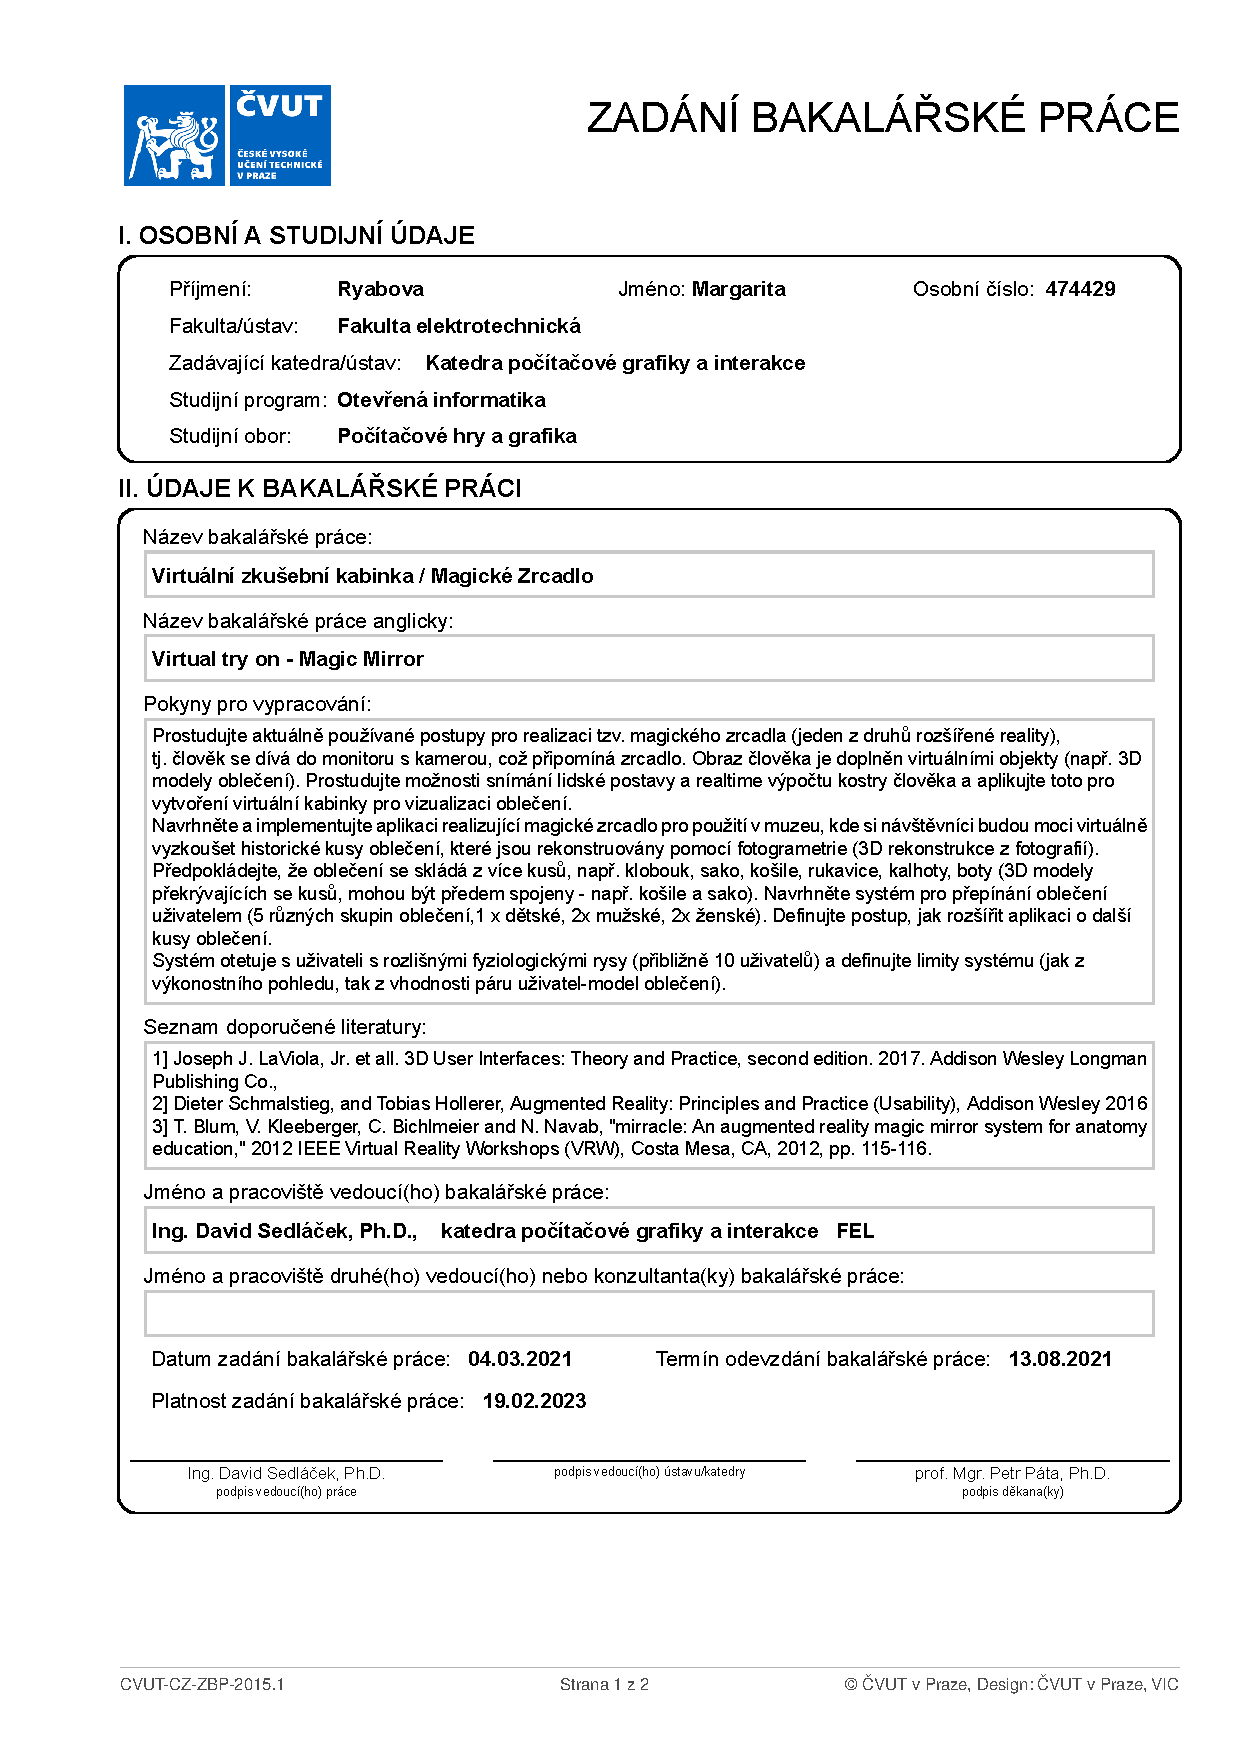
\includepdf[pages=-]{BP_task_no_signature.pdf}
%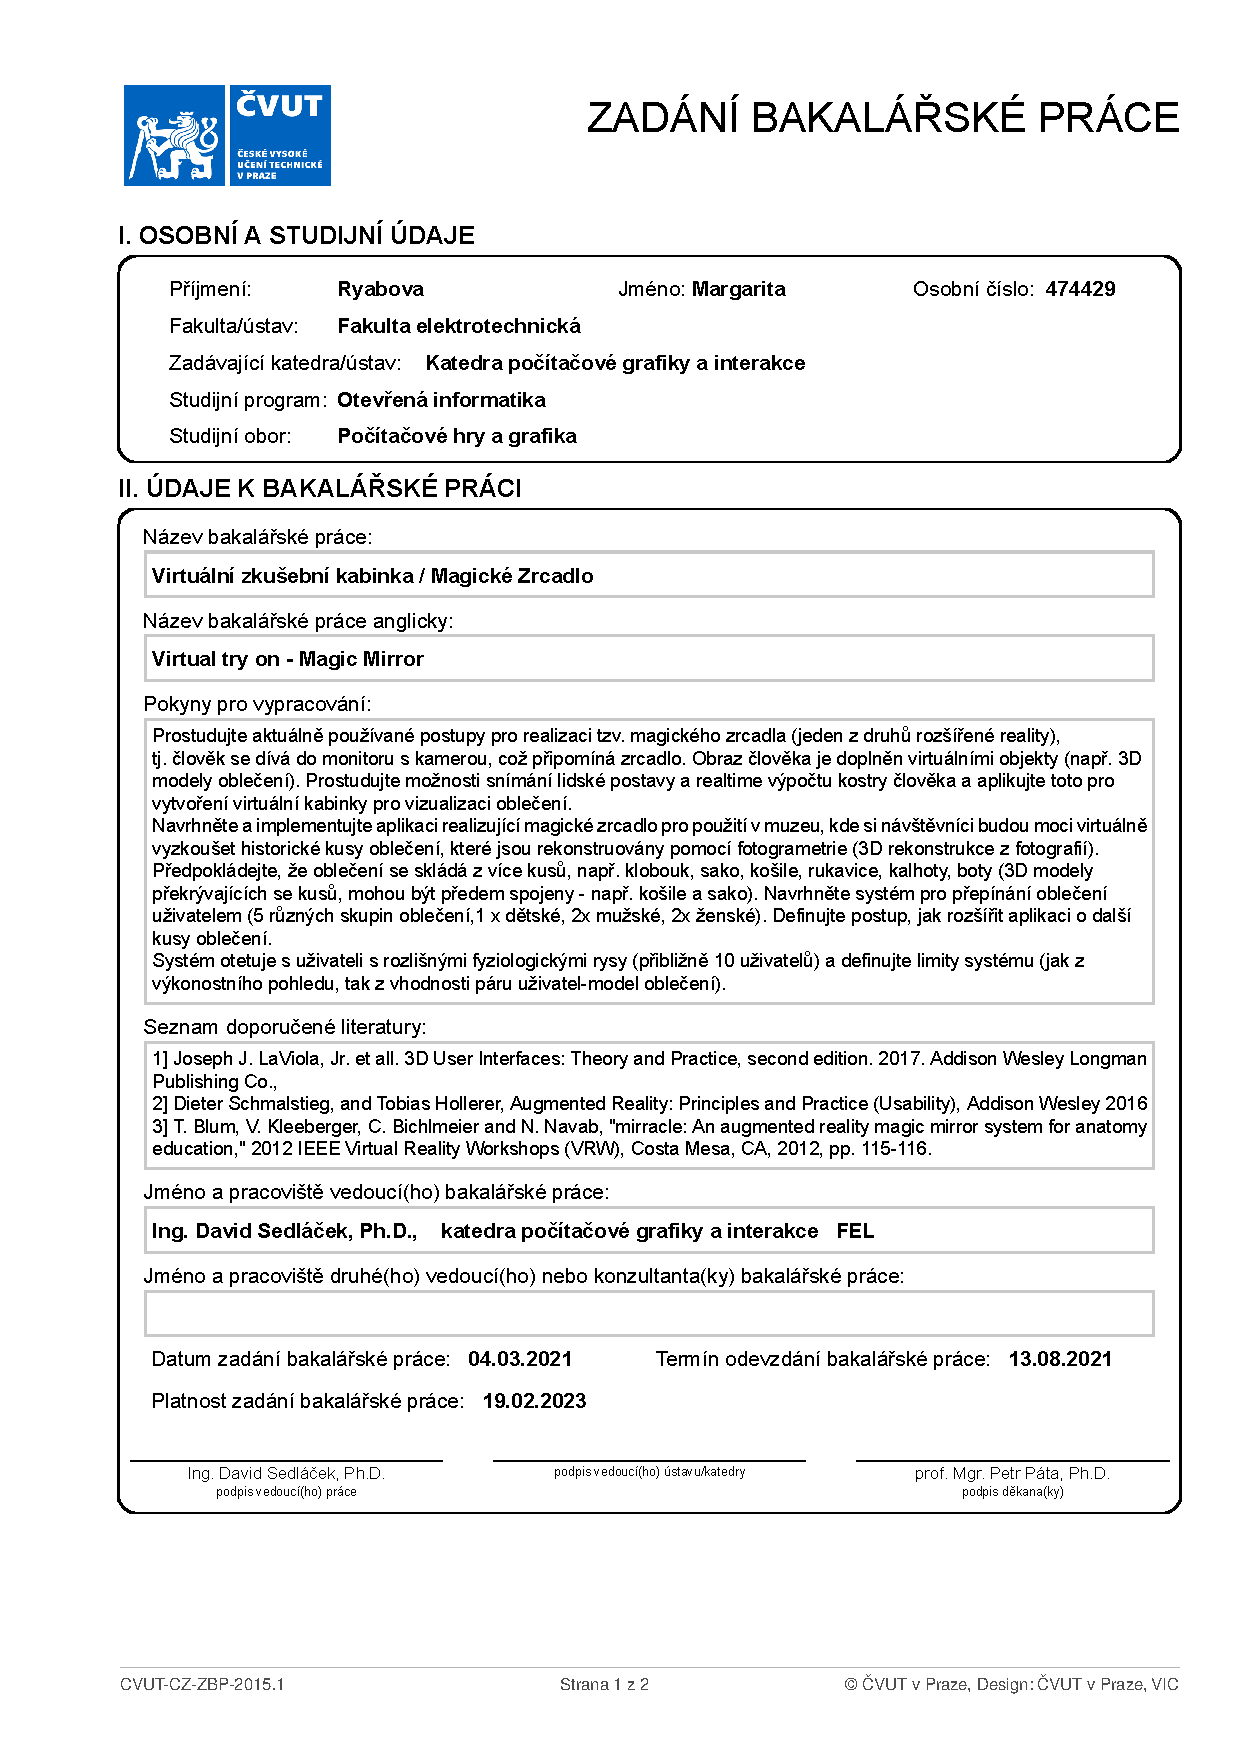
\includepdf[pages=-]{BP_task_no_signature.pdf}

% ================================================================================================%
% ================================== TITLE PAGE ==================================================%
% ================================================================================================%
\begin{titlepage}

\newcommand{\HRule}{\rule{\linewidth}{0.5mm}} % Defines a new command for the horizontal lines, change thickness here

\center % Center everything on the page
 
%----------------------------------------------------------------------------------------
%	HEADING SECTIONS
%----------------------------------------------------------------------------------------

\textsc{\LARGE Czech Technical University In Prague}\\[0.5cm] % Name of your university/college
\textsc{\large Faculty of Electrical Engineering}\\[0.5cm] % Major heading such as course name
\textsc{\large Department of Computer Graphics and Interaction}\\[1.5cm] % Major heading such as course name
\textsc{\Large Bachelor Thesis}\\[0.5cm] % Minor heading such as course title

%----------------------------------------------------------------------------------------
%	TITLE SECTION
%----------------------------------------------------------------------------------------

\HRule \\[0.4cm]
{ \huge \bfseries Virtual Try On - Magic Mirror}\\[0.4cm] % Title of your document
\HRule \\[1.5cm]
 
%----------------------------------------------------------------------------------------
%	AUTHOR SECTION
%----------------------------------------------------------------------------------------

\begin{minipage}{0.4\textwidth}
\begin{flushleft} \large
\emph{Author:}\\
Margarita {Ryabova}  \\
\end{flushleft}
\end{minipage}
~
\begin{minipage}{0.5\textwidth}
\begin{flushright} \large
\emph{Supervisor:} \\
Ing. David Sedláček, Ph.D. \\
\end{flushright}
\end{minipage}\\[2cm]

%----------------------------------------------------------------------------------------
%	DATE SECTION
%----------------------------------------------------------------------------------------

{2021}\\[2cm] % Date, change the \today to a set date if you want to be precise

%----------------------------------------------------------------------------------------
%	LOGO SECTION
%----------------------------------------------------------------------------------------


\includegraphics[width=60px, keepaspectratio]{images/CTU/ctu_logo_blue.pdf}\\[1cm] % Include a department/university logo - this will require the graphicx package

%----------------------------------------------------------------------------------------
\vfill % Fill the rest of the page with whitespace
\afterpage{\blankpage}
\end{titlepage}

% ================================================================================================%


\pagenumbering{gobble}


% ================================================================================================%
% ================================== Acknowledgements ============================================%
% ================================================================================================%


\chapter*{Acknowledgements}

\qquad Firstly, I would like to thank my supervisor Ing. David Sedláček, Ph.D. for all the suggestions
and help given during my work on this thesis. Secondly, I would like to thank the Department of Computer Graphics and Interaction of Czech Technical University in Prague for providing me with Kinect v2 device for my work on this thesis. Then, I would very much like to thank my family members for inspiring me during my study at Czech Technical University in Prague, this thesis would not have been finished without their invaluable support. Lastly, I would like to thank my close friends, who have agreed to participate in the final application testing, thank you for your priceless feedback and criticism.

\afterpage{\blankpage}


% ================================================================================================%
% ================================== Declaration ============================================%
% ================================================================================================%

\chapter*{Declaration}

\qquad I hereby declare that the presented thesis is my own work and that I have
cited all sources of information in accordance with the Guideline for adhering
to ethical principles when elaborating an academic final thesis. I acknowledge that my thesis is subject to the rights and obligations stipulated by the Act No. 121/2000 Coll., the Copyright Act, as amended, in
particular that the Czech Technical University in Prague has the right to conclude a license agreement on the utilization of this thesis as school work under
the provisions of Article 60(1) of the Act.

\bigskip

\bigskip

\noindent\begin{tabular}{lr}

In Prague on 20th of May, 2021 &  \makebox[2.0in]{\hrulefill} \\

\end{tabular}

\newpage
\mbox{}
\vfill
Czech Technical University in Prague

Faculty of Electrical Engineering

© 2021 Margarita Ryabova. All rights reserved.
 
\textit{
This thesis is school work as defined by Copyright Act of the Czech Republic.
It has been submitted at Czech Technical University in Prague, Faculty of
Electrical Engineering. The thesis is protected by the Copyright Act and its
usage without author’s permission is prohibited (with exceptions defined by the
Copyright Act).}

\textbf{ Citation of this thesis}

Ryabova, Margarita. \textit{Virtual Try On - Magic Mirror}. Bachelor’s thesis.

Czech Technical University in Prague, Faculty of Electrical Enineering, 2021. 

% ================================================================================================%
% ================================== ABSTRACT - CZ =================================================%
% ================================================================================================%

\chapter*{Abstrakt}


\qquad Hlavním cílem této práce je analyzovat možné způsoby realizace virtuální zkušební kabinky a implementovat takovou aplikaci. Na základě výzkumu bylo rozhodnuto provést implementaci pomocí Rozšiřené reality (AR) ve spojení s zařizením Kinect v2 a Unity Engine. Výsledný program byl úspěšně otestován na osobním počítači s operačním systémem Windows.

\bigskip 
\bigskip 
\textbf{Keywords:}
\keywords{Rozšiřená realita, AR, Kinect, Virtuální zkušební kabinka, Avatar, Unity, C\#, Off-Axis projekce, Inverzní kinematika, IK}



% ================================================================================================%
% ================================== ABSTRACT -EN =================================================%
% ================================================================================================%

\chapter*{Abstract}


\qquad The main goal of this thesis is to analyze the possible solutions of a virtual fitting room application and implement such an application. Based on the research, it was decided to carry out the implementation in Augmented Reality with the conjunction of Kinect v2 and Unity Engine. The final program was successfully tested on a personal computer with Windows OS.

\bigskip 
\bigskip 
\textbf{Keywords:}
\keywords{Augmented Reality, AR, Kinect, Virtual fitting room, Virtual changing room, Virtual dressing room, Avatar, Unity, C\#, Off-Axis Projection, Inverse Kinematics, IK}


% ================================================================================================%
% ================================== CONTENTS ====================================================%
% ================================================================================================%

\tableofcontents{}

% skip page numbering
\pagenumbering{gobble}


% ================================================================================================%
% ================================== BODY ========================================================%
% ================================================================================================%


% ================================================================================================%
% ================================== CHAPTER 1 ===================================================%
% ================================================================================================%

\clearpage

\pagenumbering{arabic}
\chapter{Introduction and Motivation}

% заголовок
%\section{Introduction}

%v модификации текста
%\textbf{BOLD}
%\textit{ITALIC}

% список
%\begin{itemize}
    %\item  one
   % \item two
%\end{itemize}

%

\qquad The contemporary pace of life dictates its own rules for every field, including shopping. Modern people rarely have enough time to spend on this activity, thus, the computer industry comes up with new ideas and applications to make the shopping process more effective and accessible. 


\bigskip People are increasingly fond of online shopping as it becomes possible to make quick and efficient purchases from anywhere. Distance shopping is also a better option for those who prefer to avoid crowds, which proved to be a reasonable decision during the Covid-19 pandemic. Considering the changes taking place in the world, it would be better to transfer as many activities as possible in digital format. Online shopping has another important advantage, as it gives customers more freedom of choice. Unfortunately, even the biggest offline stores are unable to store an unlimited selection of clothes in different sizes. The assortment of the store also strongly depends on the store’s location itself; sometimes a wanted item may not be available for sale in a particular city or country, which makes offline purchase impossible in this case. 

Despite the fact that online shopping seems to be a much more convenient way to buy clothes, there is a negative trait, which turns out to be decisive for many customers. Some people avoid purchasing outfits online without trying them on, as it is impossible to fully evaluate the fit or the fabric quality. Besides, it can be uneasy to pick the right size, because not every online store provides size charts, making it difficult to make the right decision. 
One of the possible solutions for the mentioned problem could be a so-called \textit{virtual fitting room application} [figure \ref{fig:virtual_fitting_example}] (also known as  \textit{virtual dressing room} or  \textit{virtual changing room}), that allows users to try on outfits virtually and receive a better picture of clothes. 

\bigskip First virtual fitting rooms appeared in the early 2000s in a number of stores, and their main purpose was to help consumers with shopping \cite{VFR_management}. The system allowed users to try on outfits instantly, making it faster for them to decide on specific items than trying the clothes on physically. As a result, the users could choose different clothing styles, sizes and colors, they could also save created outfits and compare them, to pick the most appealing one. Moreover, it was a much easier way for customers to search through the catalog and look for specific items. The \textit{Technology visibility and consumer adoption of virtual fitting rooms (VFRs): a cross-cultural comparison of Chinese and Korean consumers} by H. Lee \cite{VFR_marketing_china_korea} analyzes the popularity of virtual fitting rooms from perspective of marketing in Asian region and compares it to Western market and concludes that "the size of the VFR market is expected to grow consistently".




\begin{figure}[H]
\centering
  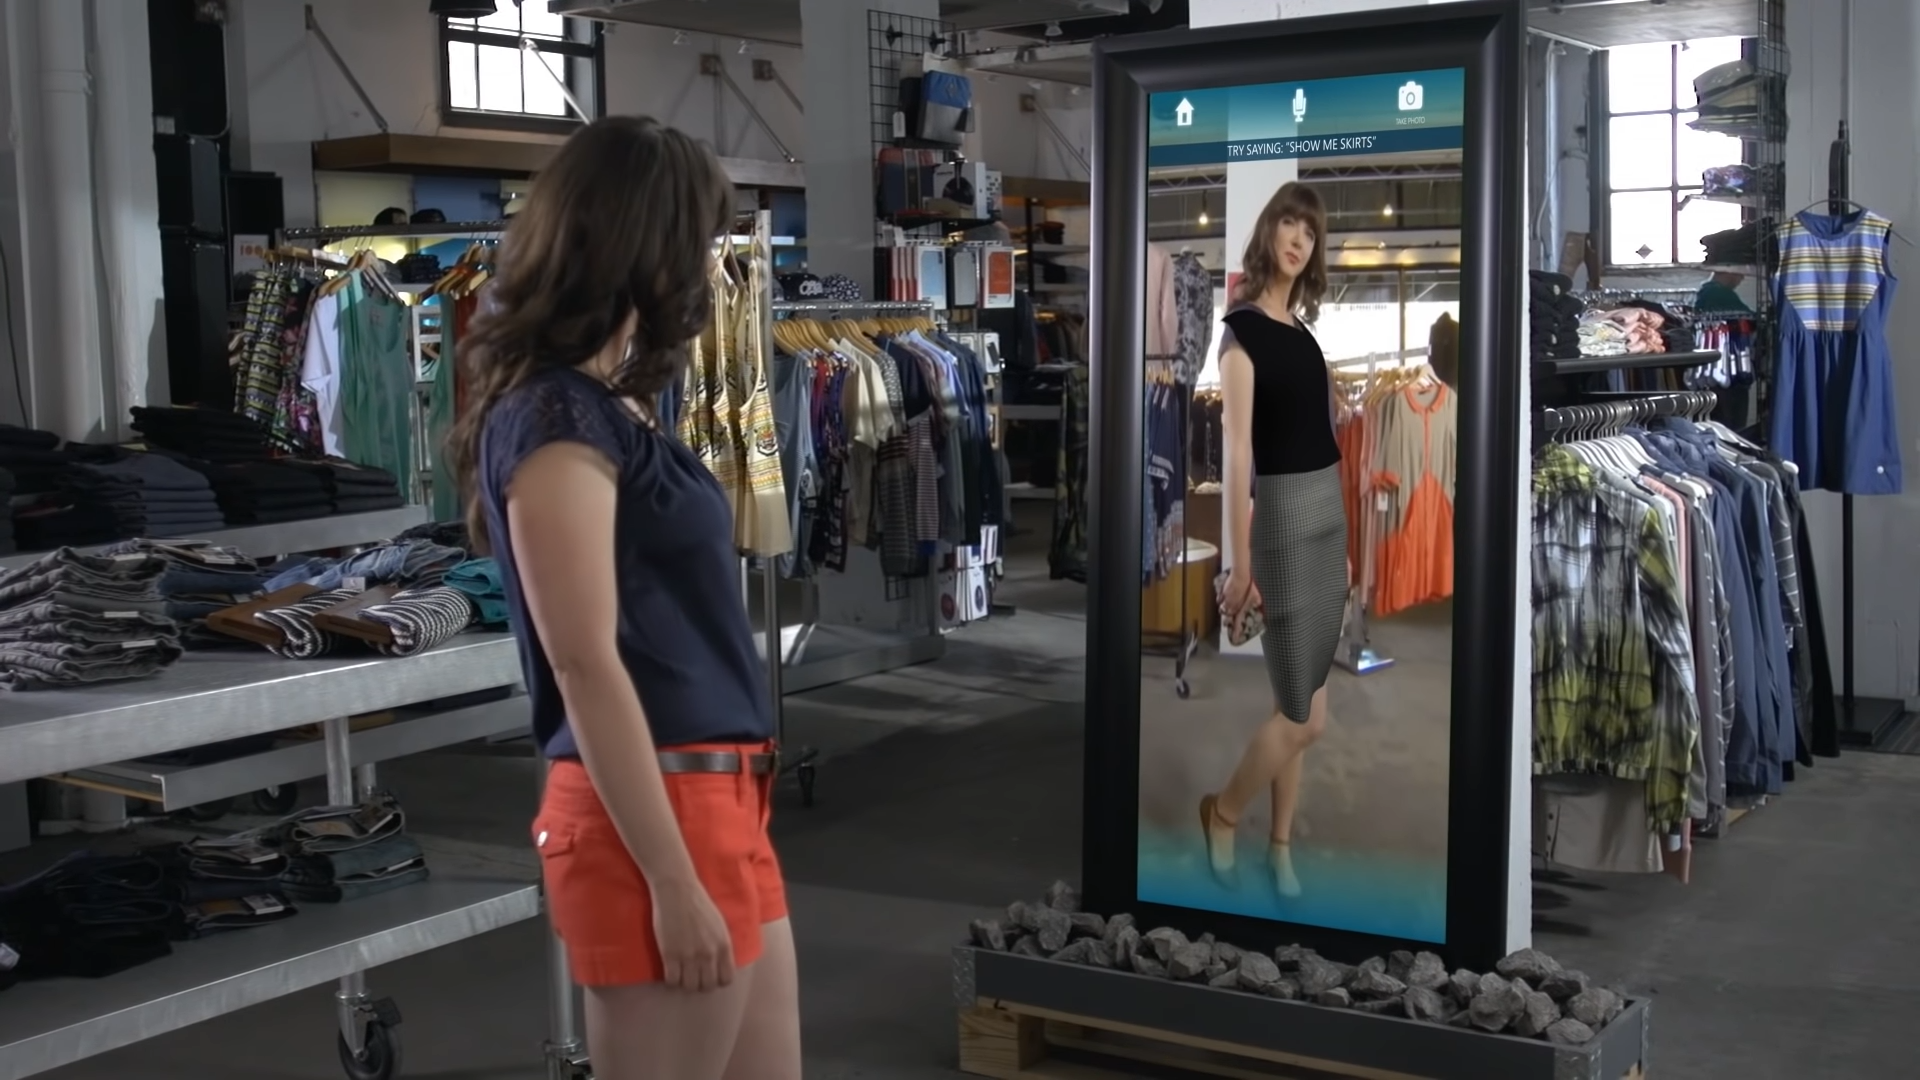
\includegraphics[width = \textwidth, keepaspectratio]{images/VFR/VFR_example_2D_2(1).png}
  \caption{Example of virtual clothes fitting in store with Microsoft Kinect \cite{kinectStoreDemo}.}
  \label{fig:virtual_fitting_example}
\end{figure}

In the last years with the development of technology it became possible to improve the virtual fitting room concept, giving the users an option to try new clothes in the comfort of home without visiting stores. This approach can be successfully combined with online sales, helping the customers to pick the most suitable items and reducing the possibility of purchase returns. The \textit{Tendency to Use the Virtual Fitting Room in Generation Y} by M. Moroz \cite{VFR_management} widely analyzes the advantages of virtual fitting rooms in online shopping sector in order to reduce the number of clothes returns. 

Such systems would address some of users’ concerns about online shopping, but not all of them. Unfortunately, the described method cannot provide users with the full idea of a clothing piece, as there is no technology to properly translate fabrics texture or quality of tailoring yet. Given this fact, virtual fitting rooms may solve this problem only partially.

Although the mentioned concept seems to be effective in marketing, the idea can be also applied in other fields. Virtual dressing rooms have a significant advantage offering the user an ability to try on any type of clothing, even the outfits, that in modern realities cannot be purchased or even manufactured. It is possible to create a historical outfit from ancient eras in digital form and offer users access to try it on. That way they will receive an experience, that cannot be repeated in real life. It is also possible to model non-existing fictional outfits that simply cannot be created in practice.

\newpage
Thus, there is another field where the use of virtual dressing rooms is becoming more and more popular: the museums create unique AR installations, allowing users to "try on" costumes from the past (for example, \cite{museumMagicMirror} and \cite{museumVFR}). Such systems in museums are still very rare at the moment, but provided that the developer gets access to 3D reconstructions of historical costumes, it will be possible for him to turn his virtual fitting room application into a system for trying on clothes from past eras.

Additionally, virtual dressing rooms can be used in clothes designing, as it would help designers to visualize their drafts and modify them easily. The program would present the general impression of the product before the manufacturing.

Lastly, such applications may be applicable for educational purposes, for example the \textit{mirracle: An augmented reality magic mirror system for anatomy education} \cite{auMagicMirror} presents the usage of a similar application for human anatomy studies.

\bigskip Virtual fitting rooms allow users to solve a number of mentioned problems, but unfortunately, this solution is not optimal. Even though the indicated method is capable of displaying outfits on top of the user’s representation, it does not present an idea of fabric quality and comfort of clothing yet.

%\begin{figure}[h!]
%\centering
%добавляет картиночку 
%\includegraphics[scale=1.7]{universe}
%\caption{The Universe}
%\label{fig:universe}
%\end{figure}


% ================================================================================================%
% ================================== CHAPTER 2 ===================================================%
% ================================================================================================%

\chapter{Problem Analysis}
\label{chapter_problemAnalysis}

\qquad There are several ways to implement the concept of a virtual changing room, to do so it is possible to apply simpler ideas and technologies or more advanced ones. This section considers and compares the realizations of these systems in 2D, 3D and augmented reality based on the research on existing applications I have done.



\section{Application in 2D}

\qquad First of all, I would like to analyze the most primitive implementations of virtual clothes fitting -  the solutions in 2D space. Let us consider the applications that allow users to put clothes on a mannequin, both the dummy and the outfits being presented in the form of two-dimensional images. In this approach, the mannequin is representing the user, playing the role of the avatar [figure \ref{fig:example_2d_1}]. Such applications are user-friendly and easy to implement, they also do not have heavy hardware demands and would work fluently on any modern device. These dress up programs are designed mainly to help customers to combine fits, prints and colors, however because the clothes are represented by flat images, it is not possible to fully convey all of the outfits’ qualities. The other issue in this concept would be “the border” between the avatar and the user, that prevents the second from imagining how the clothes will look on them. From the user's perspective, there is no connection between him and the mannequin in the mentioned solution. Nonetheless, this approach is widely used by online stores and its popularity was described in \textit{Tendency to Use the Virtual Fitting Room in Generation Y} by M. Moroz \cite[p. 242]{VFR_management}.

\begin{figure}[H]
  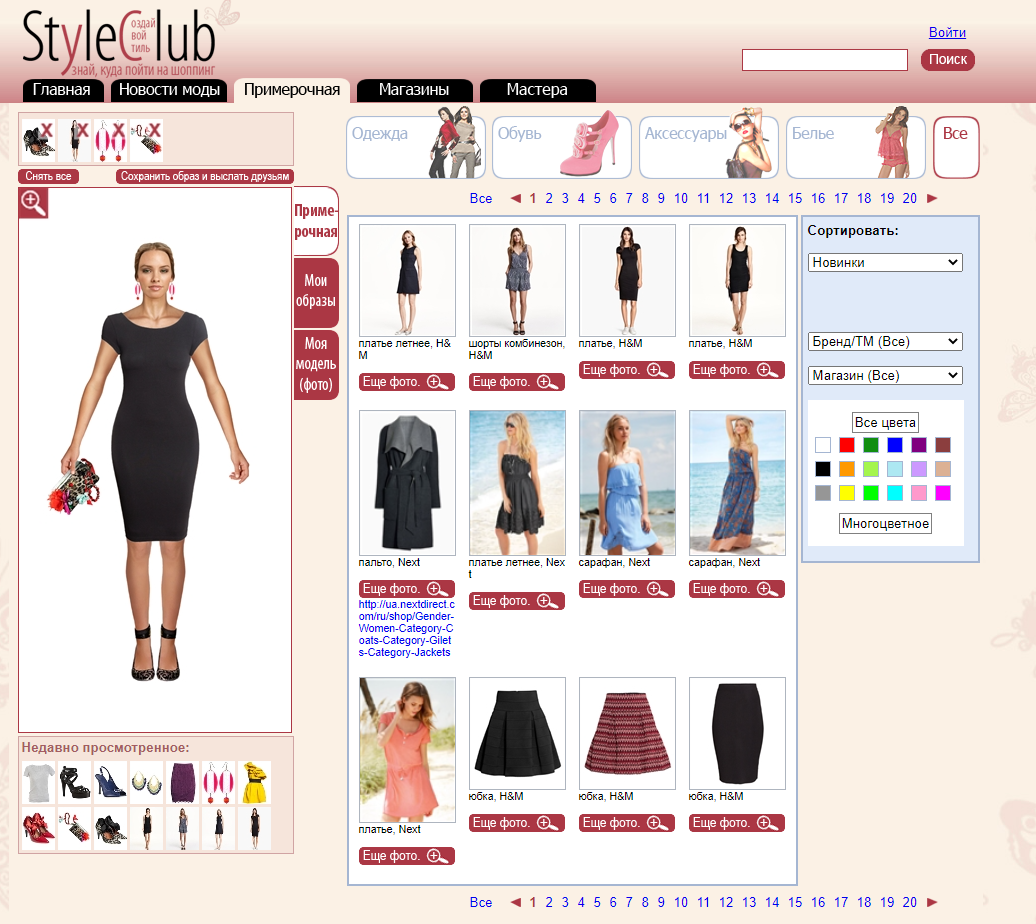
\includegraphics[width=\textwidth, keepaspectratio]{images/VFR/VFR_example_2D_1.png}
  \caption{Example of virtual clothes fitting in 2D with a standard two-dimensional avatar. Style Club web application \cite{styleclub}.}
  \label{fig:example_2d_1}
\end{figure}

\bigskip  The previously described approach can be improved by allowing the user to personalize the mannequin, for example, by using a user’s photo instead of the picture of a prepared character [figure \ref{fig:example_2d_2}]. This upgrade will solve the problem with the “facelessness” of the mannequin, making it easier for the user to associate himself with the avatar. This method will not affect the application’s performance and it will improve the “trying on” experience the user gets. This way, the customers will be able to evaluate not only the colors and designs of clothes, but also the shapes and the fits. Nevertheless, such minor changes in product design will have an impact on the core mechanics of the application. Because users’ bodies are not standardized, in this solution the developers are unable to create universal clothes that fit everyone. They would have to deform the images, that represent outfits, to match the user's constitution, and to do it right, they might need to limit the user on uploading photos with one specific pose. This, in turn, complicates the process of the application usage for the user himself.

\begin{figure}[H]
\centering
 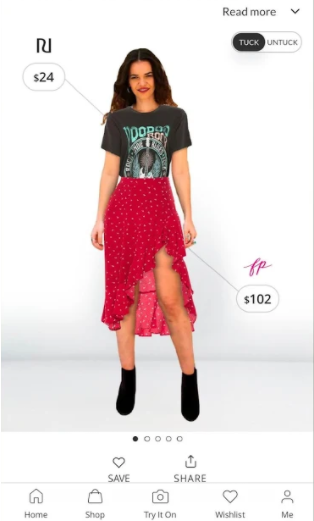
\includegraphics[height = 300, keepaspectratio]{images/VFR/VFR_example_2D_2(2).png}
 \caption{Example of virtual clothes fitting in 2D with a customized avatar, made from the user's photo. Zeekit android application \cite{zeekit}.}
  \label{fig:example_2d_2}
\end{figure}


\section{Application in 3D}
\qquad Next, let us consider the solution in 3D space. It is possible to do this in a similar way, as in the first case, but instead of using a two-dimensional mannequin, let us prepare a 3D model of the avatar and map selected clothes onto it [figure \ref{fig:example_3d_1}]. Such an approach is easy to implement, and if we compare the performance of the 2D and 3D methods, the difference would not be dramatic. Even though the 3D solution requires better hardware than the previous application, it will still easily work on the modern platforms. The three-dimensional approach would let customers examine clothes meticulously, as they would be able to rotate the avatar and inspect the outfits from different points of view. Unfortunately, the users may be still unattracted to the idea of dressing up a mannequin that has nothing in common with them.

\begin{figure}[H]
\centering
\begin{subfigure}{\textwidth}
  \centering
  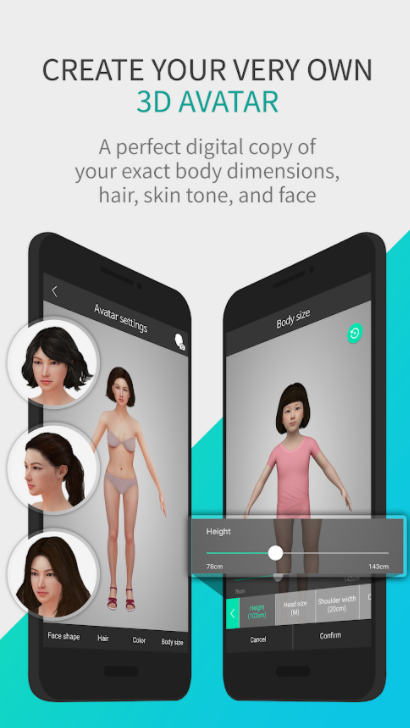
\includegraphics[width=.45\textwidth , keepaspectratio]{images/VFR/VFR_example_3D_1(1).png}
  \label{fig:sub1_example_3d_1_a}
\end{subfigure}%
\begin{subfigure}{\textwidth}
  \centering
  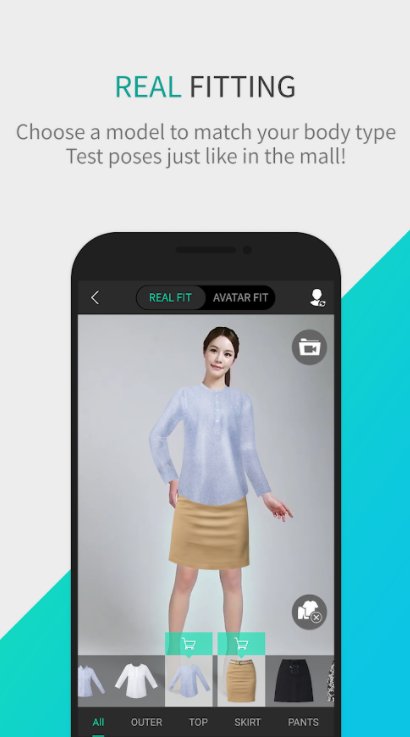
\includegraphics[width=.45\textwidth , keepaspectratio]{images/VFR/VFR_example_3D_1(2).png}
  \label{fig:sub2_example_3d_1_b}
\end{subfigure}
\caption{Example of virtual clothes fitting in 3D with a standard three-dimensional avatar. FIT'N SHOP android application \cite{fitnshop}.}
\label{fig:example_3d_1}
\end{figure}

\bigskip This approach can also be improved by allowing the user to dress up not a foreign avatar, but a three-dimensional copy of himself. To do so, the application would need to scan the user and create a 3D model from the received data. The resulting model will replace the standard mannequin in the application, helping the user to associate himself with the customized avatar easily [figure \ref{fig:example_3d_2}]. In this approach, the concept of a virtual dressing room starts to open up. The solution would guide users to pick clothes' fits, designs and probably even recommend sizes. However, the process of user scanning in this solution is not a simple operation and if done wrong, the resulting model turns out unusable. It should also be mentioned that the quality of a scanned model is typically much worse than the quality of a manually prepared avatar, especially if the resolution of used images is low. The second down side of this solution is the need to dynamically deform 3d meshes of clothes to match the user's model (that was not necessary with a standard mannequin). Doing so would be much more complicated than editing 2D images in the one of the previously mentioned solutions.



\begin{figure}[H]
  
  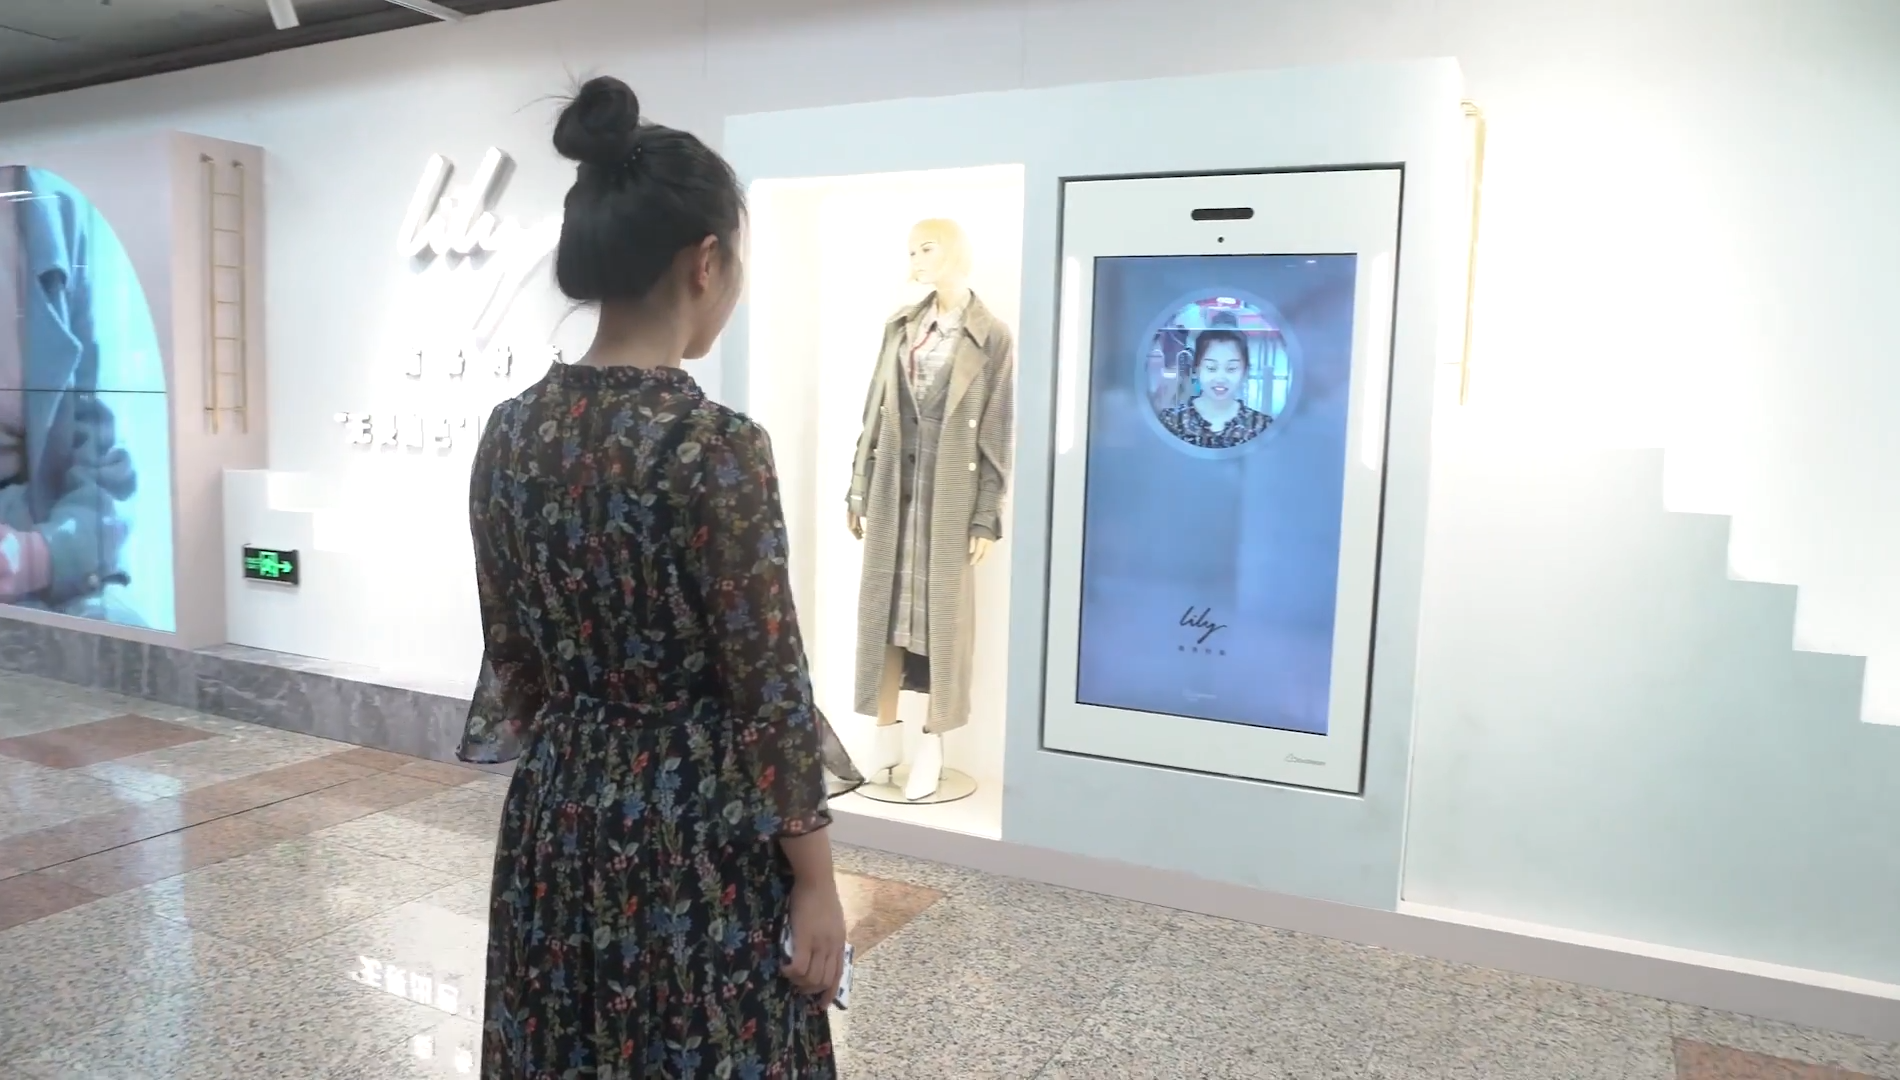
\includegraphics[width=\textwidth, keepaspectratio]{images/VFR/VFR_example_3D_2(1).png}
  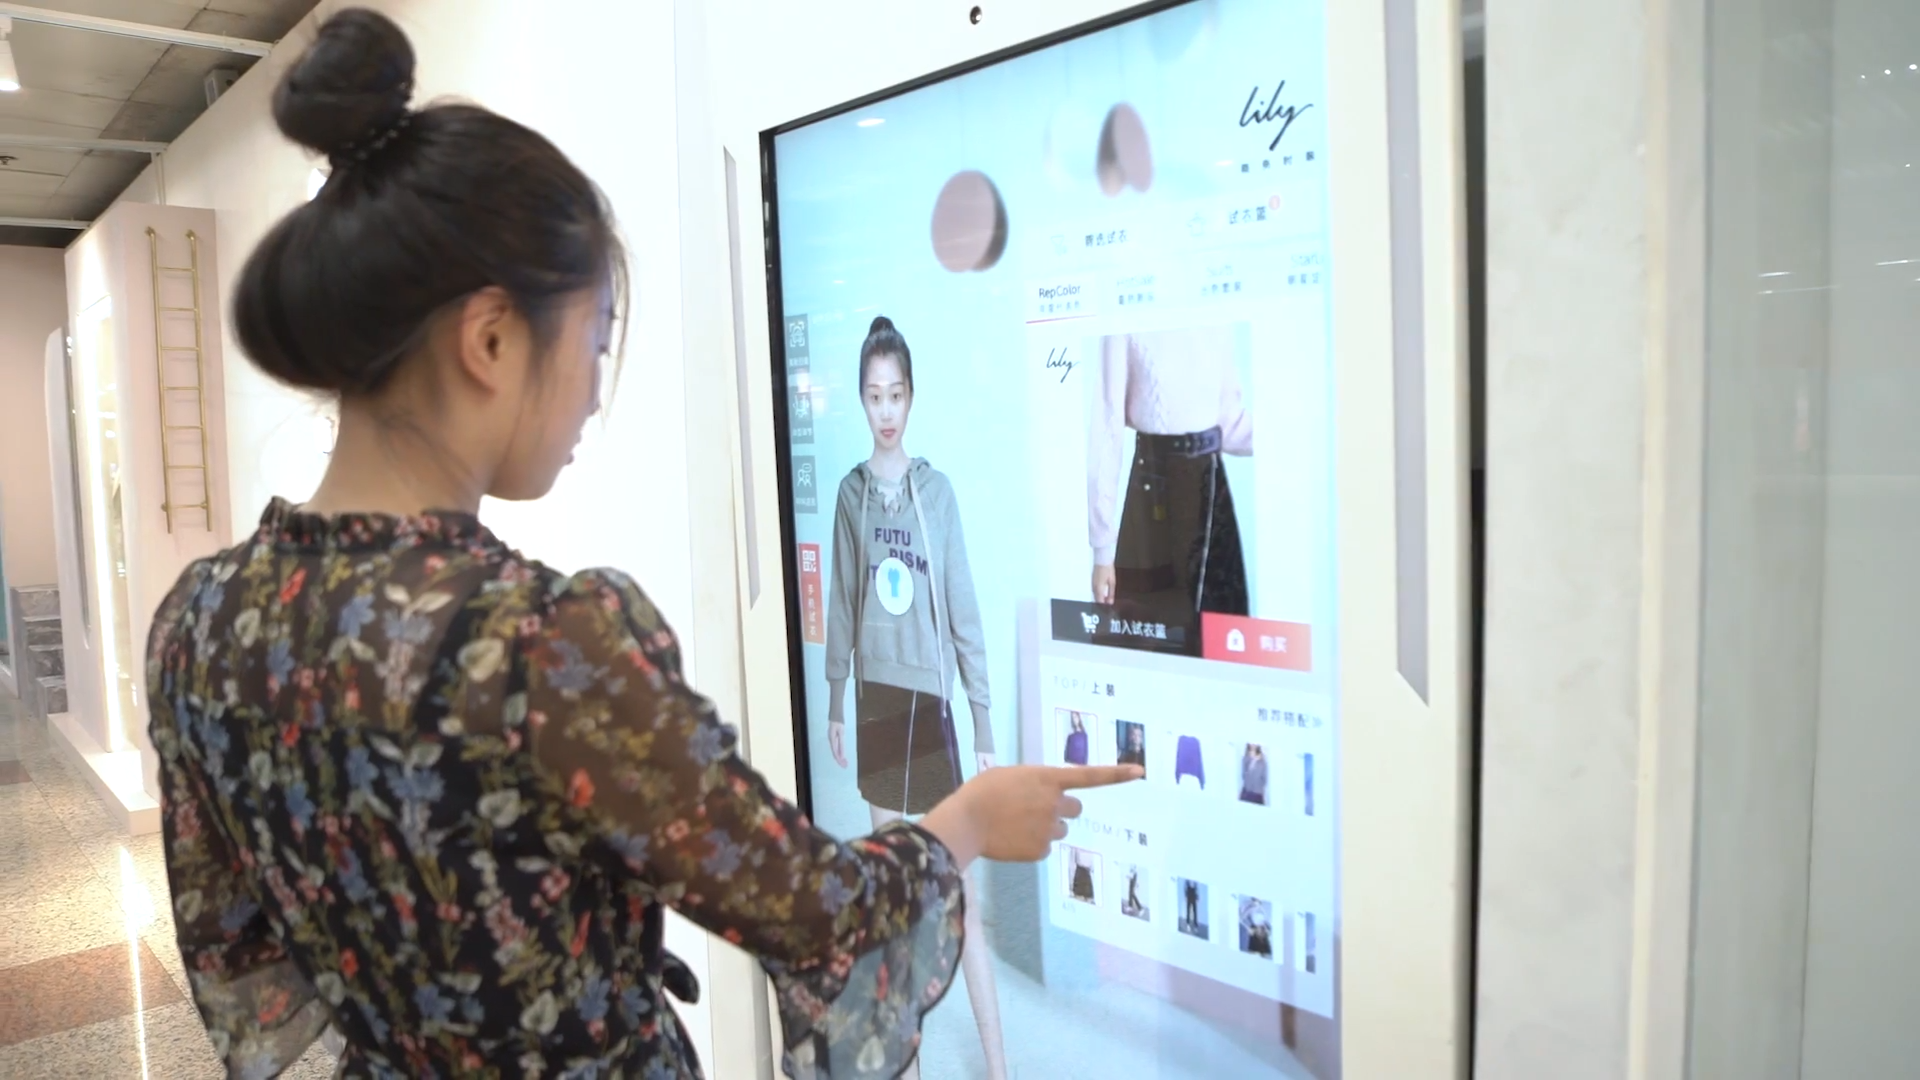
\includegraphics[width=\textwidth, keepaspectratio]{images/VFR/VFR_example_3D_2(2).png}
  \caption{Example of virtual clothes fitting in 3D with a customized avatar made with user scanning. Virtual fitting room of brand Lily at in Shanghai metro. Source video: \cite{ARvirtualFittingYoutubeVideo}.}
  \label{fig:example_3d_2}
\end{figure}

\section{Application in AR}
\label{section_AR}
\qquad The last option we will consider allows to make the virtual fitting process even more natural. To make this happen, we will not force the user to dress up an artificial avatar or convince the user that the avatar is similar to him. Instead, let us project the clothing directly onto the user's image [figure \ref{fig:example_ar}]. It can be done by implementing an interactive mirror-like application with a clothes try-on feature. The user sees himself in the display as if the content on the screen was the mirrored reality, but augmented by an interface, that allows the user to pick specific clothes and map them on his “reflection” in the monitor. To do so, the application will require a device with a camera, that will send captured data to the program for a further processing. 

\begin{figure}[H]
  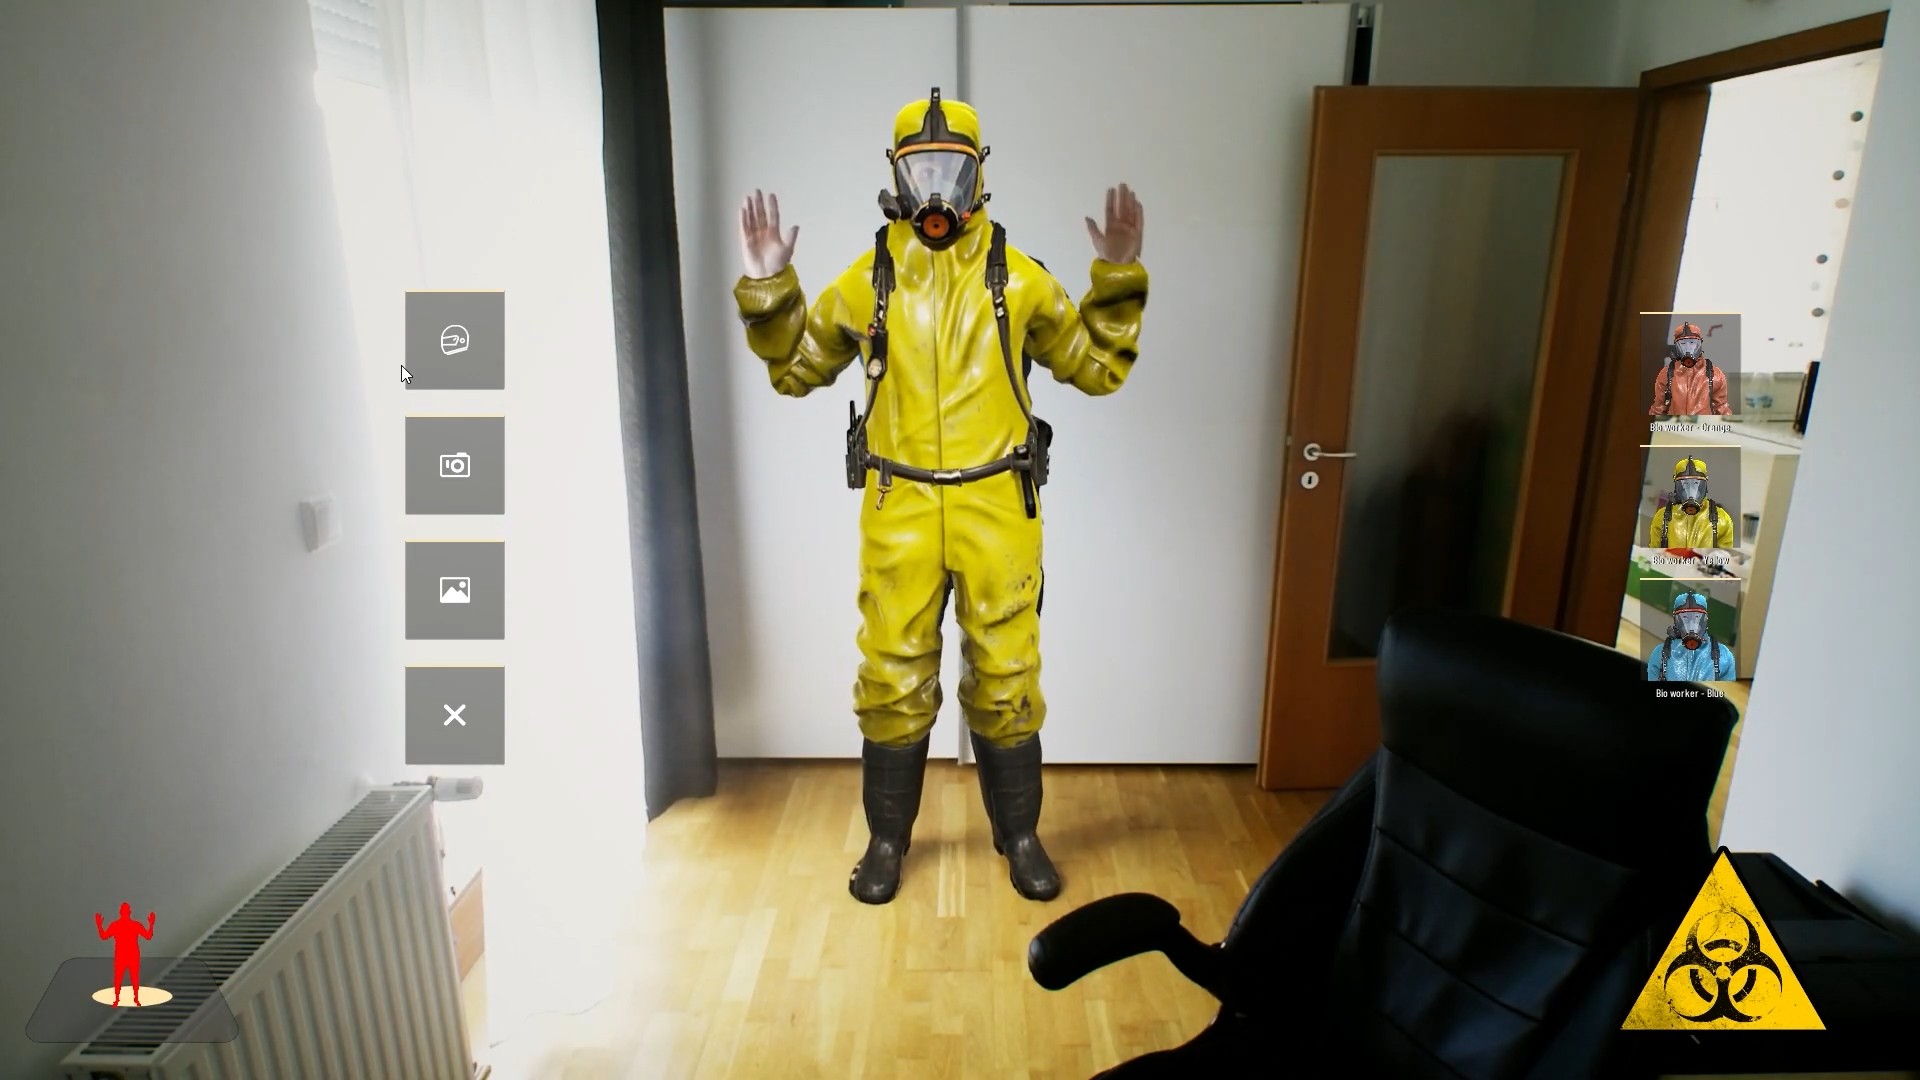
\includegraphics[width=\textwidth, keepaspectratio]{images/VFR/VFR_example_AR.png}
  \caption{Example of virtual clothes fitting in AR. Fitnect Kinect application \cite{Fitnect}.} 
  \label{fig:example_ar}
\end{figure}


\bigskip Such a concept can be implemented with use of a classic web camera. This device is easily accessible, most people own a web camera at home, so they will not need to purchase special equipment to make the application function. Unfortunately, most of the web cameras can not have the ability to capture high quality videos or to trace the movement well. However, this is not the main problem of this solution, because in case of using the web cameras for movement tracing it would be necessary to implement the whole motion capture system. Such algorithms are complicated and will require much time and knowledge to implement.

The other possibility is to implement the application on smartphones, that are also accessible in our daily life, but tend to have a rather better quality of captures, compared to web cameras. Unfortunately, the body tracking problem is still present in this case and the developers would have to deal with it on their own.

The last option we will consider is the use of one of Microsoft Kinect devices. The Kinect devices have a significant advantage over the previously discussed options, because they were designed to deal with body tracking tasks primarily. The devices are supported by an SDK, specially made for development of the programs and games, that rely on body tracking. The devices offer a complete implementation of motion capture and depth and color records. The downside of this solution is that Kinect is not a popular device and not every person has one at home. It is also not a cheap system and people might not be interested in buying it only to try out one application. Nonetheless, this specific technology is popular between developers, who implement virtual dressing rooms and there is a high number of materials on this topic, such as:

\begin{itemize}
   
    
    \item The \textit{Experiences in the Development of an Augmented Reality Dressing Room} by U. Erra \cite{VFR_experiences_AU_Unity} characterizes an implementation of a virtual dressing room application with Kinect technology and Unity Engine, explaining the possible instruments that can be used for this approach.
    
    \item The \textit{An Efficient Magic Mirror Using Kinect} by J. Uddin \cite{VFR_efficient_magic_mirror} proposes a concept of real time virtual dressing room with gesture based interaction techniques.
    
    \item The \textit{Virtual Dressing Room Application} by A. Masri \cite{vfrApp} shares an implementation of such application using Windows Presentation Foundation and contains useful approach on clothes adjustment.
    
    \item The \textit{Augmented  Reality  Platforms  forVirtual  Fitting  Rooms} by  I.  Pachoulakis  and  K.  Kapetanakis \cite{auFittingRooms} compares Kinect for Windows to Asus Xton Pro Live and analyzes already existing AR virtual fitting room applications.


    \item The \textit{Augmented Reality Principles and Practice} by D. Schmalstieg and T. Höllerer \cite{ARpp} as well mentions a virtual dressing room to be an interesting example of Augmented Reality applications.
\end{itemize}


\section{Conclusion}
\qquad Based on the research, I came to the conclusion that the ideal option would be to implement the virtual dressing room application using AR technology. Of all the options given, this implementation seems the closest one to the user's everyday life, using such a system would make clothes fitting more natural. Choosing between web cameras, smartphones and Kinect, I opted for the latter device, since it has the best functionality and motion capture accuracy to complete the task and is ready for development.



% ================================================================================================%
% ================================== CHAPTER 3 ===================================================%
% ================================================================================================%
\chapter{Solution plan}
\label{chapter_solutionPlan}
\qquad This chapter contains a detailed solution to the problem of virtual clothes fitting in augmented reality using Microsoft Kinect. For this thesis, I used a Kinect v2 in conjunction with the official Kinect SDK\cite{KinectSDKv2}. 
First of, I have started with a brief analysis of the device key features, secondly, I decided on a game engine to be used for the task solution. Next, I have analyzed the mirror projection that would provide a simulation of the reflection effect. Afterwards I have decided on ways to visualize the user and outfits. Lastly, I have reviewed the possible ways to implement user interactions.


\section{Overview of Kinect key features}
\label{section_Kinect}
\qquad Microsoft Kinect v2 [figure \ref{fig:kinecteSensors}] is a sensing device “composed by a RGB camera with resolution of 1920×1080 pixels, an infrared camera with resolution of 512×424 pixels and an infrared emitter”\cite{kinectV2VisionSystem}. The device provides access to images from infrared and color cameras, a depth map, as well as to the position of the user's body (coordinates of his joints).
\begin{figure}[H]
  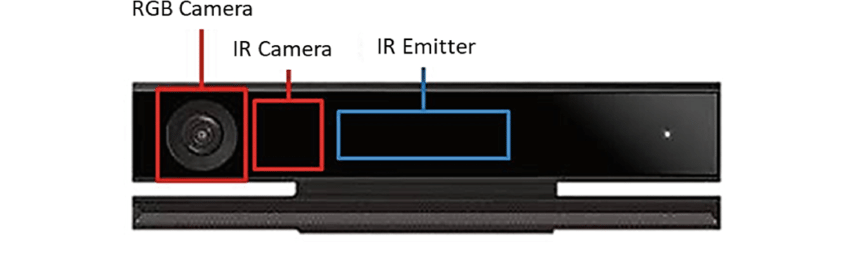
\includegraphics[width=\textwidth, keepaspectratio]{images/Kinect_sensors.png}
  \caption{The Kinect v2 sensor front with cameras and emitter positions\cite{kinectV2VisionSystem}.}
  \label{fig:kinecteSensors}
\end{figure}

 The mentioned data can be used in development of projects that require body tracking. It can be easily done with help of an official Microsoft Kinect SDK that contains all necessary libraries and lets developers work with Kinect’s data in different programming languages and game engines. The device has proven to be used in many different fields (for example, in robotics and medicine \cite{kinectV2VisionSystem}\cite{auMagicMirror}), even though it was developed as a gaming controller.

\section{Game Engine as an application basis}
\label{section_Engine}
 \qquad It is clearly not an optimal solution to develop a new engine for the given task, as there already are great engines compatible with Kinect. For further implementation I had to decide what third-party engine to use to make the work as effective as possible. 
 
\bigskip Unity3d Game Engine \cite{unity3dHome} is a well documented gaming engine, that is popular among game developers. Because of this fact, there is a significant number of studying materials such as books, articles, and tutorials (official ones and the others, made by enthusiasts). The existence of official Microsoft support of Kinect on Unity made this option the most suitable for our implementation. 
 
  Unreal Engine \cite{UnrealEngineHome} is a well-known alternative to Unity, but in case of this thesis it was not a proper option, as it is not supported by Microsoft and there is no official SDK, that provides developers to work with Kinect on this engine. On the other hand, there is a Kinect 4 Unreal project \cite{Kinect4Unreal} that provides the necessary instruments to start developing with these two components. The mentioned API puts limits on developers, allowing them to use it for free only for low-budget projects; otherwise, the developers have to purchase a licence. The number of available tutorials and materials for this topic is much smaller, than in case of Unity, that is why the previous engine seems to be a better option.
 
  It was also possible to use other less popular engines for the implementation, but in this case it would require certain effort in connecting Kinect to the workspace. For efficiency of the solution, I have decided to avoid such low-level settings.
	
\bigskip  Based on the research, Unity engine was the ideal option for the given task, as it provides stable work with Kinect sensors and a large amount of studying materials on similar topics.



\section{Mirror simulation}
\label{section_Camera}
 \qquad In the project I was planning to create a mirror-like version of a virtual fitting room. To do so, I had to consider projecting the content of the application onto the monitor in the specific way. 
 
\bigskip Normally, if we look into a mirror from different angles, we are able to see reflections of the opposite sides of our surroundings. This is the type of projection that is not used in most of the applications and games on a daily basis, because there is no need to implement it that way. Most of the time the developers apply a classic perspective projection, that in calculations does not consider the user's position according to the monitor or the angle at which the user is looking at the screen. Generally, the standard perspective projection assumes that the user is located right in front of the display, looking at its center \cite{offaxisKooima}. However, the thesis task required a different approach, in which new projection deforms the content of the screen based of the user’s position. “This behaviour may be achieved by using the off-axis perspective technique to simulate distortion when the viewpoint is shifted relative to the mirror plane”\cite{offaxisKooima}.

\bigskip The off-axis projection principles are discussed and explained in the next chapter as a part of the implementation process [\ref{offaxis}]. 

\section{Data visualization}

\label{section_Virtual_Ref}
 \qquad Let us assume that we recieve the data from the Kinect and visualize it in the 3D scene with a camera set up. After applying  the projection matrix on the camera’s content, the result of such transformation is displayed on the screen. Such output is a reflection of the environment that the Kinect is capturing. Let us call the final result of this pipeline a \textit{virtual reflection}. 

\bigskip Because I have already found the projection solution in the previous section, to create a virtual reflection I only needed to discover a way to visualize the data Kinect collects. There are several approaches to solve this problem, each of them has its own advantages and disadvantages. This section reviews the possible solutions and compares them with each other.
	
 The first way to solve the task of data visualization is to combine a 2D image from the Kinect RGB camera and map a 3D outfit on top of it. Such an approach is easy to implement, as the camera output is used as a base of the visualization. However this solution conflicts with the primary task of mirror simulation. Because the image is taken directly from the camera output, the perspective projection on captured frames will stay fixed. For the mentioned reasons, this method would not work with mirror simulation, but it could be used to represent captured data without mirror-like deformation [figure \ref{fig:example_ar}].

 The second approach that could be potentially applied in this work is a concept of a point cloud [figure \ref{fig:example_pointcloud}].
“A point cloud is a set of data points in space. The points represent a 3D shape or object. Each point has its set of X, Y and Z coordinates“\cite{wikipediaPointCloud}. It is possible to create the point cloud from Kinect output data and apply a projection transformation on it.

 Even though this solution is the most suitable for the given task, it also has significant disadvantages. Firstly, the final rendered image looks grainy, as infrared sensor resolution is limited, which may look unpleasant from the user's perspective. Secondly, the processed data is not filling the display most of the time, except for the situation, when the position of the virtual camera and the position of real sensor match. 


\begin{figure}[H]
    \centering
    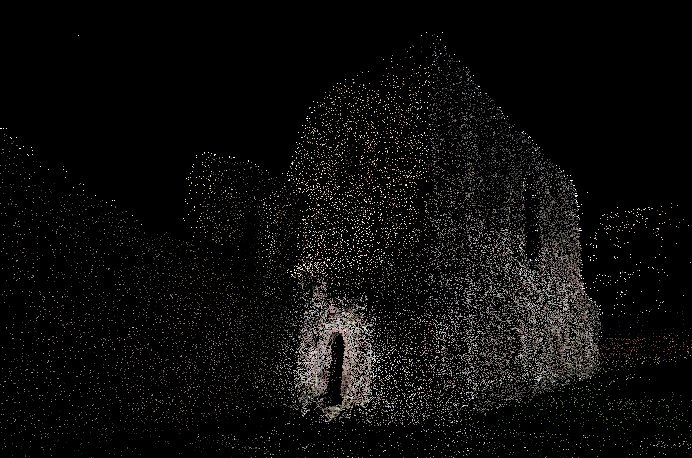
\includegraphics [width=\textwidth] {images/PointCloud.png}
    \caption{Example of a point cloud, image source: \cite{pointCLoud_image}.}
    \label{fig:example_pointcloud}
\end{figure}





\section{Outfit visualisation and mapping}
\label{section_Outfit_visual}
%\begin{itemize}
    %\item  one
   % \item two
%\end{itemize}

 \qquad In most of the virtual fitting rooms there is a user’s avatar in the scene, the picked clothes map onto this avatar. In the case of an AR application, I had to map the outfits directly onto the user’s image. 
It is possible to pretend that this is happening, while using an avatar in the background, but not rendering it. This is why I have decided to place the clothes on the avatar, that would be animated by user's movements but never rendered. With this approach only the clothes will remain on the screen. Furthermore, an invisible avatar could be used as a stencil to hide those parts of clothing that should not be visible.

\bigskip Since Kinect provides a set of the user’s joints, it is possible to position the avatar in virtual space and mimic the user's pose. However, there issues that would have to be fixed [figure \ref{fig:IK_usage}]:
\begin{itemize}
    \item the proportions of the user’s body in general do not match the proportions of the avatar
    \item due to limitations of the Kinect sensor the lengths of the user’s limbs in provided data may vary from frame to frame
\end{itemize}

The solution to these problems would be a use of inverse kinematics for consistent animation of the avatar \cite{upbodyIK}.

Unity has a built-in IK implementation but it is not entirely clear which algorithm was used to achieve it; from the documentation it is seen, that the algorithm is implemented in native code and I could not find any specific information on the algorithm itself. Moreover, due to its focus primarily on games, it has a number of disadvantages in case of the given task:

\begin{itemize}
\item unity IK can only be applied to arms (brachial bone and forearm) and legs (thigh and shin)
\item access to avatar bones is only possible through the Mecanim system
\item animator component is needed and all manipulations should be provided inside OnAnimatorIK method
\end{itemize}


Although the limitations of the built-in IK system could be overcome, in the thesis I have decided to use my own implementation of inverse kinematics, as it allows fine tuning and does not operate on other systems, such as Animator and Mecanim. As a result, in case of this thesis it was ideal to implement IK from scratch, the custom implementation must have the following advantages: 
\begin{itemize}
\item IK chains include hands and feet
\item IK not only for the limbs but also for the spine 
\end{itemize}


\bigskip In interactive applications (such as games), inverse kinematics is calculated with iterative heuristic methods, due to the ease of implementation and the low cost of computation \cite{IKtechniques}.
“The most popular heuristic algorithms are: Cyclic Coordinate Descent (CCD), and Forward And Backward Reaching Inverse Kinematics (FABRIK)” \cite{wikipediaIK}.
It was possible to use one of the two algorithms in the implementation, let us briefly characterize both of them.

\bigskip Cyclic Coordinate Descent (CCD) operates with rotation angles to reach target position.  However it is necessary to implement constraints to achieve more realistic animation. The algorithm has further advantages and disadvantages [\ref{CCD_pro_con}]:



\begin{table}[H]
\begin{tabularx}{\linewidth}{>{\parskip1ex}X@{\kern4\tabcolsep}>{\parskip1ex}X}
\toprule
\hfil\bfseries Pros
&
\hfil\bfseries Cons
\\\cmidrule(r{3\tabcolsep}){1-1}\cmidrule(l{-\tabcolsep}){2-2}

%% PROS, seperated by empty line or \par
\begin{itemize}
    \item simple to implement 
    \item extremely fast algorithm, provides a linear-time complexity in the number of degrees of freedom \cite{IKtechniques}
    \item returns a numerically stable solution \cite{IKtechniques}
\end{itemize}

&

%% CONS, seperated by empty line or \par

\begin{itemize}
    \item difficult to implement for multiple end effectors \cite{IKtechniques}
    \item often produces unrealistic animation \cite{IKtechniques}
    \item suffers from erratic discontinuities \cite{IKtechniques}
    \item the closer a joint is to the end of the chaint, the more it bends \cite{IKtechniques}
    \item found solution is not optimal, not suitable for physically correct simulation
\end{itemize}

\\\bottomrule
\end{tabularx}
\caption{Pros and cons of Cyclic Coordinate Descent heuristic algorithm}
\label{CCD_pro_con}
\end{table}




\bigskip Forward And Backward Reaching Inverse Kinematics (FABRIK) relies on previously calculated state of a chain of joints and manipulates with joints positions. FABRIK analysis [\ref{FABRIK_pro_con}]:



\begin{table}[H]
\begin{tabularx}{\linewidth}{>{\parskip1ex}X@{\kern4\tabcolsep}>{\parskip1ex}X}
\toprule
\hfil\bfseries Pros
&
\hfil\bfseries Cons
\\\cmidrule(r{3\tabcolsep}){1-1}\cmidrule(l{-\tabcolsep}){2-2}

%% PROS, seperated by empty line or \par
\begin{itemize}
    \item simple to implement 
    \item “computational cost for each joint per iteration is low” \cite{IKtechniques}
    \item if the target is in range, the algorithm always returns a solution \cite{IKtechniques}
    \item returns smooth motion without erratic discontinuities \cite{IKtechniques}
    \item the closer a joint is to the root of the chaint, the more it bends \cite{IKtechniques}
    \item can be easily modified to solve a task with multiple end effectors \cite{IKtechniques}
\end{itemize}

&

%% CONS, seperated by empty line or \par

\begin{itemize}
    \item constraints implementation is more complicated than in CCD \cite{IKtechniques}
    \item found solution is not optimal, not suitable for physically correct simulation
\end{itemize}

\\\bottomrule
\end{tabularx}
\caption{Pros and cons of Forward And Backward Reaching Inverse Kinematics heuristic algorithm}
\label{FABRIK_pro_con}
\end{table}




\section{User interaction}
\label{section_UI}
 \qquad Interactive programs need to be controlled by the user in some way. In case of this project, the user should be able to select the outfit and, if necessary, adjust its mapping.
 
  Most applications use classic input interfaces: keyboard, mouse or controller. Kinect provides the ability to use the entire body of the user as a "controller", this idea eliminates the need to set up the stand with classic input devices in front of the virtual fitting room. Instead, the user will navigate through the interface using gestures.
 
  I have decided to implement both techniques: the primary way of interaction would be using a computer mouse, and the additional way would be using simple gestures for navigation and picking clothes. The gestures would be based on simple "raise hand" or "grab" actions to make the navigation through the UI natural and intuitive, as suggested in \cite{practicalAR}[p.214]. 
  


\section{Conclusion}
\label{section_problemAnalysys_Conclusion}
 \qquad The given solution plan contains main terms and ideas used in the implementation process. Some approaches had to be modified to correspond to the given task.













% ================================================================================================%
% ================================== CHAPTER 4 ===================================================%
% ================================================================================================%
\chapter{Implementation}
\label{chapter_Implementation}

\qquad This chapter presents in detail the process of implementing each of the approaches mentioned in the last chaper.

\section{Off-Axis Projection}
\label{offaxis}

\qquad In the vast majority of games and 3d applications it is enough to rely on the default camera object provided by an engine or framework. However in the case of simulating reflection in a magic mirror application, I had to consider a special type of projection. The following explanation is heavily based on \textit{Generalized Perspective} \cite{offaxisKooima} by Robert Kooima, \textit{Off-axis projection in Unity} \cite{offaxisUnityDeBrisis} by Michel de Brisis and \textit{Implementation of Generalized Perspective Projection on the Unity} \cite{offaxisUnityKazuya} by Hiruma Kazuya.


\bigskip The Unity3d camera class produces a set of matrices used for further processing in the rendering pipeline in order to translate points from world coordinates to screen coordinate system. But I could not use them as they put the user's eyes position directly in front of the screen.

\bigskip Let us assume the plane with points $p_a$, $p_b$, $p_c$ defines the screen. Let us suppose that a set of some vectors $v_r$, $v_u$ and $v_n$ is an orthonormal basis of the screen space [figure \ref{fig:offaxis_1}].

\begin{figure}[H]
\centering
\begin{subfigure}{\textwidth}
  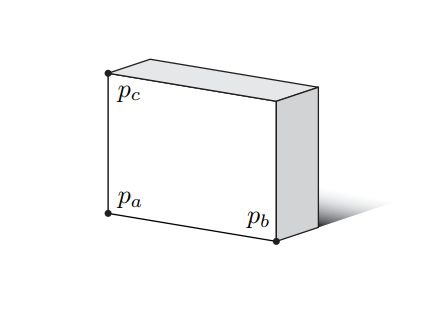
\includegraphics[width=.4\textwidth, keepaspectratio]{images/Scemas/pa_pb_pc_pd.png}
  \label{fig:pa_pb_pc_pd}
\end{subfigure}%
\begin{subfigure}{\textwidth}
  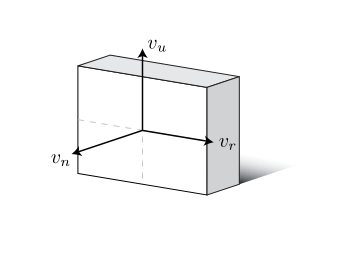
\includegraphics[width=.4\textwidth, keepaspectratio]{images/Scemas/Vn_Vu_Vr_basis.png}
  \label{fig:vn_vu_vr}
\end{subfigure}
\caption{Screen space definition \cite{offaxisKooima}.}
\label{fig:offaxis_1}
\end{figure}

\newpage

These vectors can be calculated from the following formulas\cite{offaxisKooima}:
 \[v_r = \frac{p_b - p_a}{\norm{p_b - p_a}}\]
\[v_u = \frac{p_c - p_a}{\norm{p_c - p_a}}\]
\[v_n = \frac{v_r \times v_u}{\norm{v_r \times v_u}}\]

 In general the eye position $p_e$ is projected on the center of the screen [figure \ref{fig:on_axis}]. Let us call this point a \textit{screen space origin}. According to the task for this thesis, I need to implement a mirror-like projection, and to do so, I had to let the eye position not be fixed. From now on let us suppose that screen space origin can be located anywhere on the screen plane [figure \ref{fig:off_axis}].
 
 
 
\begin{figure}[H]
\centering
\begin{minipage}{.5\textwidth}
    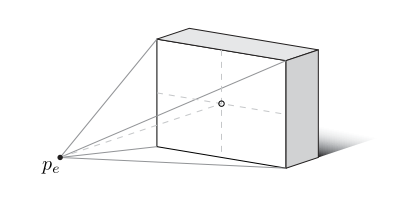
\includegraphics[width=\linewidth, keepaspectratio]{images/Scemas/on_axis.png}
    \caption{On-Axis projection \cite{offaxisKooima}.}
    \label{fig:on_axis}
\end{minipage}%
\begin{minipage}{.5\textwidth}
    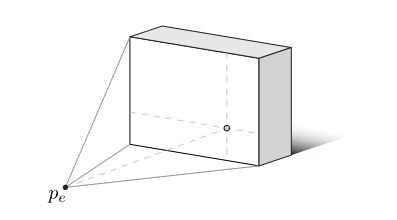
\includegraphics[width=\linewidth, keepaspectratio]{images/Scemas/off_axis.png}
    \caption{Off-Axis projection \cite{offaxisKooima}.}
   \label{fig:off_axis}
\end{minipage}%
\caption{On-Axis and Off-Axis projections \cite{offaxisKooima}.}
\label{fig:offaxis_1}
\end{figure}


  Let us divide the sides of the plane according to the screen space origin and name the sides \textit{l, r, b, t} [figure \ref{fig:offaxis_3}]. Let us also add a parameter \textit{d}, that stores the distance from $p_e$ to the screen-space origin, and parameters  \textit{n, f} for distances from $p_e$ to near and far clipping planes.
  
\begin{figure}[H]
\centering
    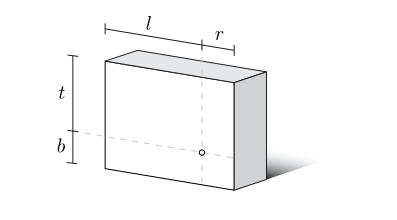
\includegraphics[width=.6\textwidth, keepaspectratio]{images/Scemas/screen_space_distance.png}
    \caption{Screen divison and parameters definition \cite{offaxisKooima}.
    \label{fig:offaxis_3}}
 
\end{figure}

 Assume non-unit vectors from $p_e$ to the corners of the screen( $v_a$, $v_b$, $v_c$) [figure \ref{fig:offaxis_4}].

\begin{figure}[H]
\centering
  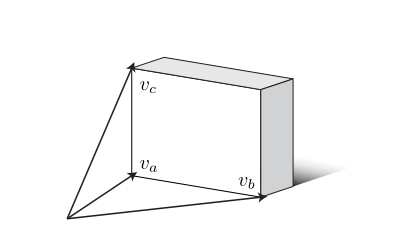
\includegraphics[width=.6\textwidth, keepaspectratio]{images/Scemas/va_vb_vc.png}
  \caption{Vectors $v_a$, $v_b$, $v_c$ introduction \cite{offaxisKooima}.  
  \label{fig:offaxis_4}}
\end{figure}

        \[v_a = p_a - p_e\]
        \[v_b = p_b - p_e\]
        \[v_c = p_c - p_e\]
        
        These parameters are calculated in the following way:
        \[d = -(v_n \cdot v_a)\]
        \[l = (v_r \cdot v_a) \frac{n}{d}\]
        \[r = (v_r \cdot v_b) \frac{n}{d}\]
        \[b = (v_u \cdot v_a) \frac{n}{d}\]
        \[t = (v_u \cdot v_c) \frac{n}{d}\]
        
        And use them in Perspective projection matrix\cite[p.~4]{offaxisKooima}:
        \[ P =
        \begin{vmatrix}
            \frac{2n}{r-l}  & 0              & \frac{r+l}{r-l}  & 0                 \\
            0               & \frac{2n}{t-b} & \frac{t+b}{t-b}  & 0                 \\
            0               & 0              & -\frac{f+n}{f-n} & -\frac{2fn}{f-n}  \\
            0               & 0              & -1               & 0
        \end{vmatrix}
        \]

        Projection plane orientation matrix:
        \[ M^T =
        \begin{vmatrix}
            v_{rx} & v_{ry} & v_{rz} & 0\\
            v_{ux} & v_{uy} & v_{uz} & 0\\
            v_{nx} & v_{ny} & v_{nz} & 0\\
            0      & 0      & 0      & 1
        \end{vmatrix}
        \]
        
        And view offset transformation matrix:
        \[ T =
        \begin{vmatrix}
            1 & 0 & 0 & -p_{ex}\\
            0 & 1 & 0 & -p_{ey}\\
            0 & 0 & 1 & -p_{ez}\\
            0 & 0 & 0 & 1
        \end{vmatrix}
        \]
        
        
        Finally, all previous matrices are composed together:
        
        \[
            P' = P \times M^T \times T
        \]
        
        
    On practice, it was used in Unity to define \verb|worldToCameraMatrix| and \verb|projectionMatrix| fields of camera component. To determine the position of the camera, I used the position of the user's head reflected from the surface of the projection frame.
    
    Assuming that the Kinect sensor is in the origin of the coordinates, by moving and rotating the projection frame in the scene, it is possible to match its position with the relative position of the screen and the sensor in the real world. This will achieve the effect of a "magic mirror".

        
        
\begin{figure}[H]
\centering
\begin{subfigure}{\textwidth}
  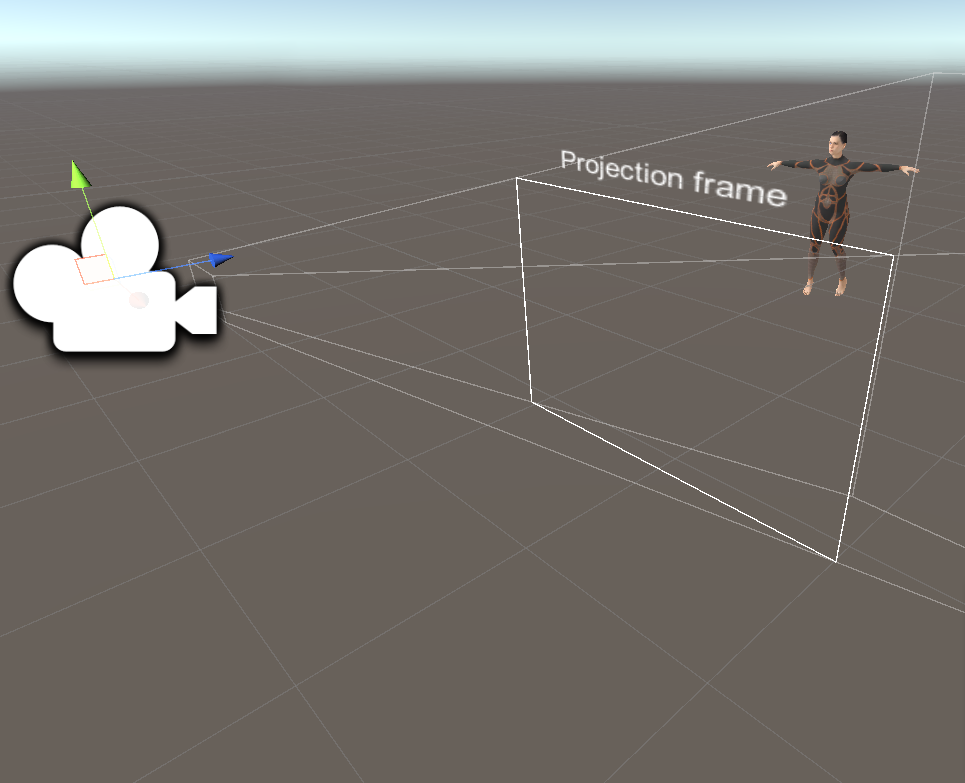
\includegraphics[width=.45\textwidth, keepaspectratio]{images/OffAxis/offaxis_demo_1.png}
\end{subfigure}%
\begin{subfigure}{\textwidth}
  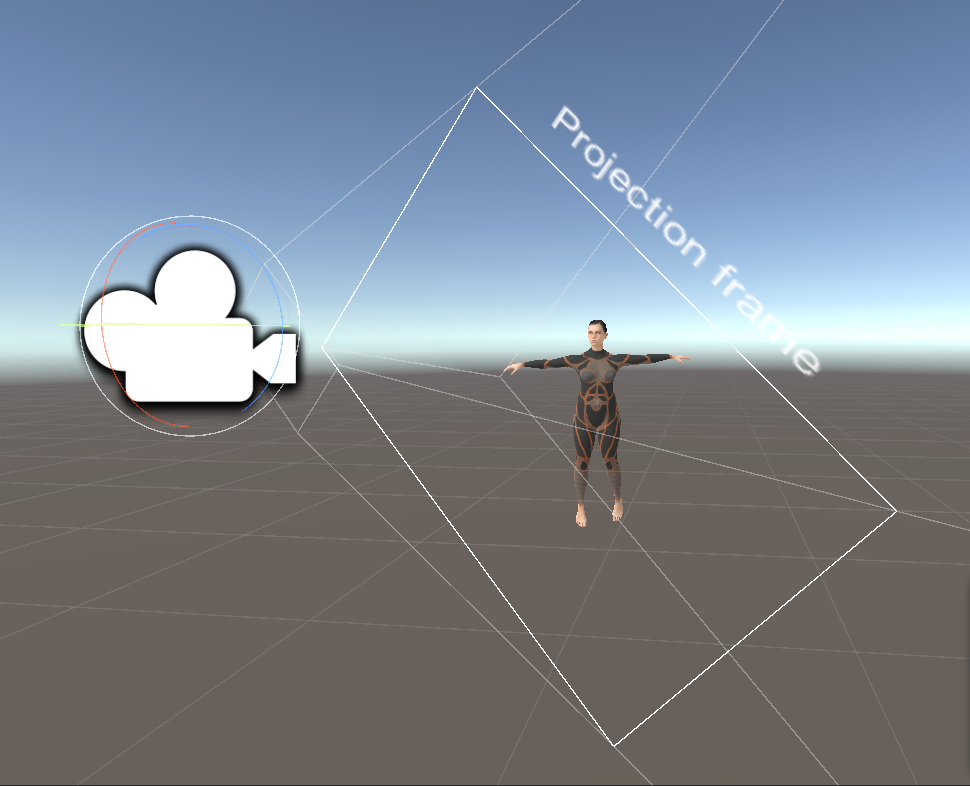
\includegraphics[width=.45\textwidth, keepaspectratio]{images/OffAxis/offaxis_demo_2.png}
\end{subfigure}
\caption{Projection frame in Unity.}
\label{fig:offaxis_demo}
\end{figure}
        
        
        
        
        
        
        

\section{Kinect Data Visualization}
\subsection{2D visualization}
\qquad To accomplish this basic visualization method it was enough to ensure that the user's avatar is covering the user on the image obtained from the color camera of the sensor. To achieve this, I have placed a flat plane with a texture to the 3D scene and updated the texture with the output from the color camera of the Kinect every frame.
With the correct placement of the camera, the plane and the avatar, the outfits will be covering the user's body from the camera output, creating the illusion that the user is wearing the clothes.



 \begin{figure}[H]
\centering
\begin{subfigure}{\textwidth}
  \centering
  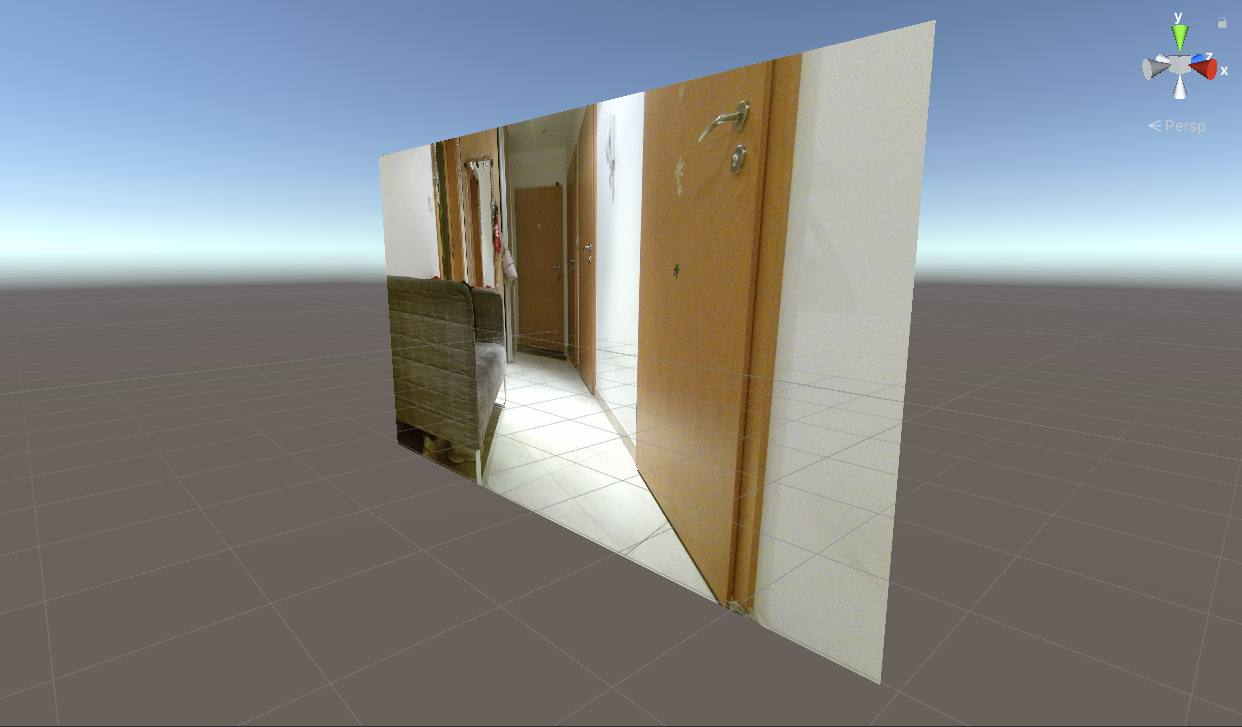
\includegraphics[width=.45\textwidth , keepaspectratio]{images/ClothesDemos/Screenshot 2021-05-13 173422.png}
\end{subfigure}%
\begin{subfigure}{\textwidth}
  \centering
  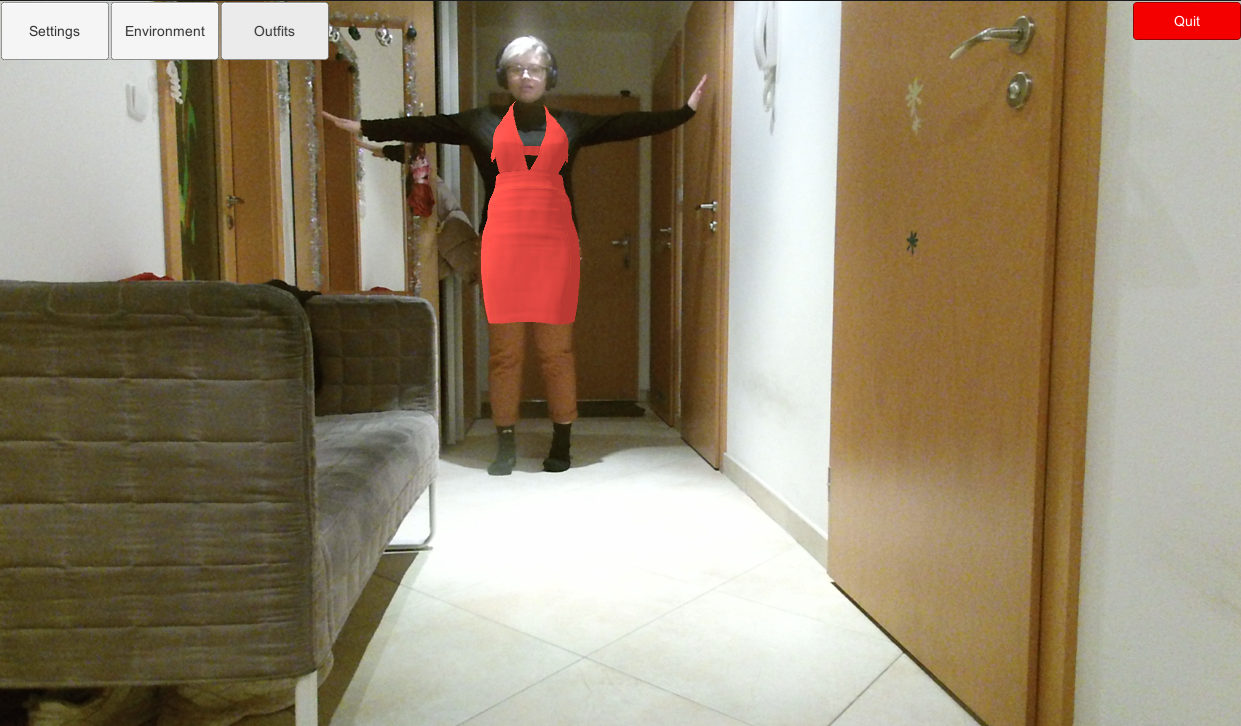
\includegraphics[width=.45\textwidth , keepaspectratio]{images/ClothesDemos/Screenshot 2021-05-14 185933 (1).png}
\end{subfigure}
\caption{2D visualization demonstration.}
\label{fig:example_2d_vis}
\end{figure}






\subsection{Point cloud visualization}
\label{section_pointCLoud}

\begin{figure}[H]
\centering
\begin{subfigure}{\textwidth}
  \centering
  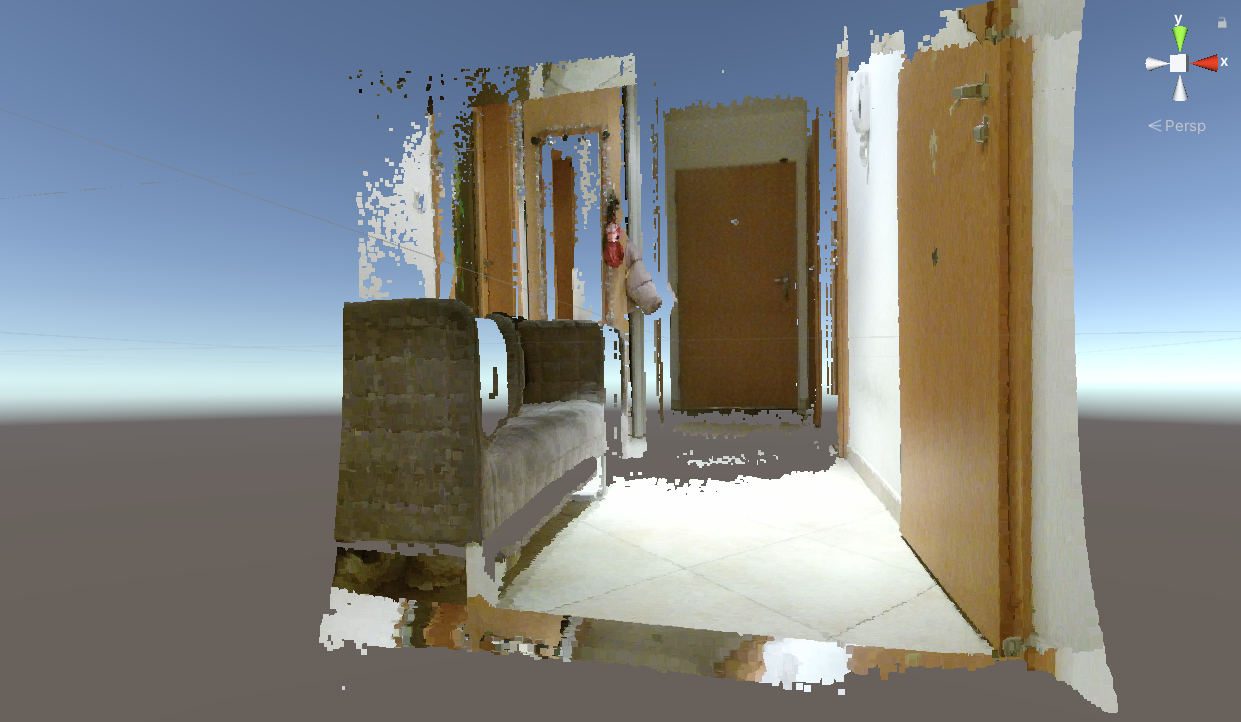
\includegraphics[width=.45\textwidth , keepaspectratio]{images/ClothesDemos/Screenshot 2021-05-13 173650.png}
\end{subfigure}%
\begin{subfigure}{\textwidth}
  \centering
  \includegraphics[width=.45\textwidth , keepaspectratio]{images/ClothesDemos/Screenshot 2021-05-13 174257.png}
\end{subfigure}
\caption{Point cloud demonstration.}
\label{fig:pc_demo_1}
\end{figure}

 \qquad To create a three-dimensional visual representation of Kinect data I decided to implement a point cloud [figure \ref{fig:pc_demo_1}]. It was done by using Kinect SDK \textit{DepthFrameReader} and \textit{ColorFrameReader} classes to acquire and process data from sensors and \textit{CoordinateMapper} class to project that data on 3D space.
   \begin{table}[H]
   
            \centering
            \begin{tabular}{| c | c | c |} 
                \hline
                                    & Resolution    &   Framerate   \\
                \hline
                Color camera        & 1920x1080     &       30      \\
                \hline
                Infrared camera     & 512x424       &       30      \\
                \hline
            \end{tabular}
            
            \caption{Kinect v2 sensor resolutions \cite{kinctV1V2Comparison}.}
            \label{tab:kinectv2Capabilities}
           
        \end{table}

 \bigskip Let us first describe the way Kinect stores the data of each frame [table \ref{tab:kinectv2Capabilities}]. The frame is captured by the infrared camera has resolution of 512× 424 pixels, and Kinect internally calculates depths for each pixel in the form of a one-dimensional array.
 
 Next, the point depth buffer was then converted using the \textit{CoordinateMapper} into two new buffers: a 3D point array and a color camera image space coordinate array to use as UV coordinates.


The data from the first buffer were used as the coordinates of the Point cloud points, and the data from the second buffer were used to sample the color of this point from the image output of the color camera.
To turn the points into squares, I used a geometry shader. This allowed me to achieve filling the gaps between the points by adjusting the size of the squares.

\bigskip To further improve the image quality, I had to increase the number of points in the point cloud. However, for the number of points greater than what Kinect v2 can provide, it was necessary to interpolate their positions, this required additional processor resources. Additionally, I kept in mind that if the desired number of points is not a multiple of the original number of points, the implementation would be complicated. 

To implement such approach I have decided to put the coordinate buffer data and the UV buffer data into textures. That way, the interpolation was done in the shader by sampling the texture.

% ==== Data in textures =================



 \bigskip It is a common practice to save normals as a texture. Acting on the same principle, I decided to write 3D space coordinates and UVs into textures. To avoid loss of precision, the texture format which stores color in float values (such as ARGBFloat or RGFloat) was chosen.

\begin{figure}[H]
\centering
  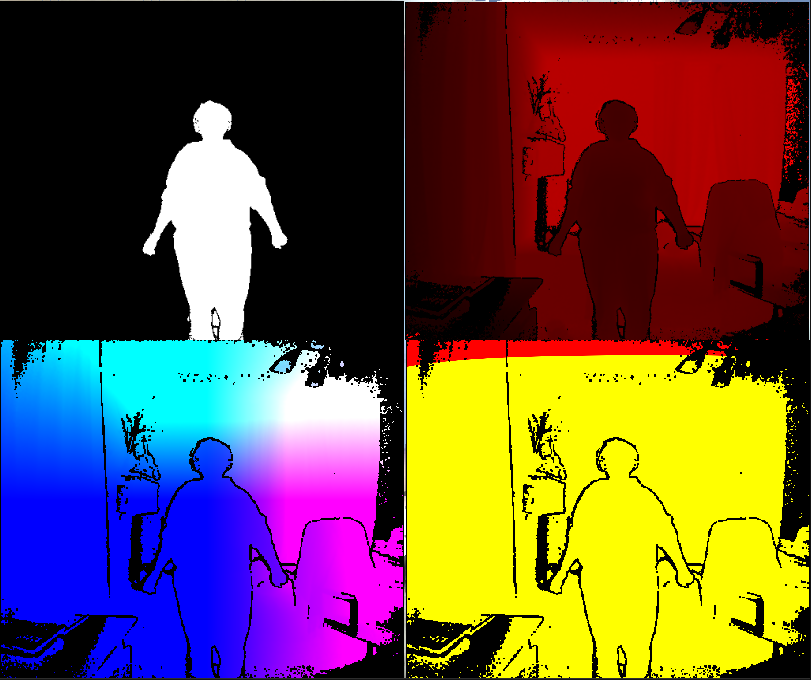
\includegraphics[width=\textwidth , keepaspectratio]{images/ClothesDemos/Screenshot 2021-05-14 184422.png}
\caption{Body indexes, Depths, Positions, UVs as they will be rendered as textures}
\label{fig:pc_demo_2}
\end{figure}

Next, to get a position and a UV coordinate of a point [figure \ref{fig:pc_demo_2}], the coordinates for sampling are calculated as 

\begin{align*}
x &\equiv idx \mod width \\
y &\equiv idx   \div   width \\
\end{align*}
where $idx$ is the point index and $width$ is the number of points horizontally.


Thus, it was possible to set an arbitrary number (bigger, less or equal to the original number) of points in the point cloud. They will be evenly distributed and their coordinates will be interpolated between the values that Kinect can provide [figure \ref{fig:pc_demo_3}].


\begin{figure}[H]
\centering
\begin{subfigure}{\textwidth}
  \centering
  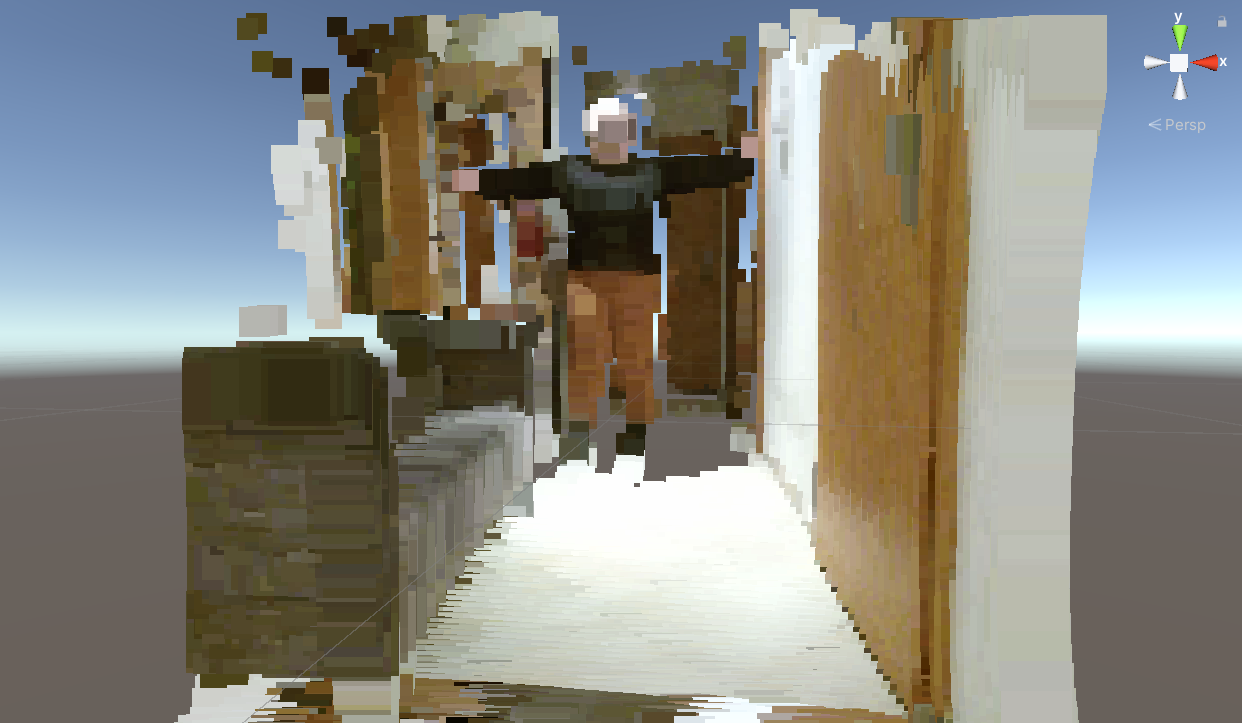
\includegraphics[width=.45\textwidth , keepaspectratio]{images/pointCloud/Screenshot 2021-05-14 211444_.png}
\end{subfigure}%
\begin{subfigure}{\textwidth}
  \centering
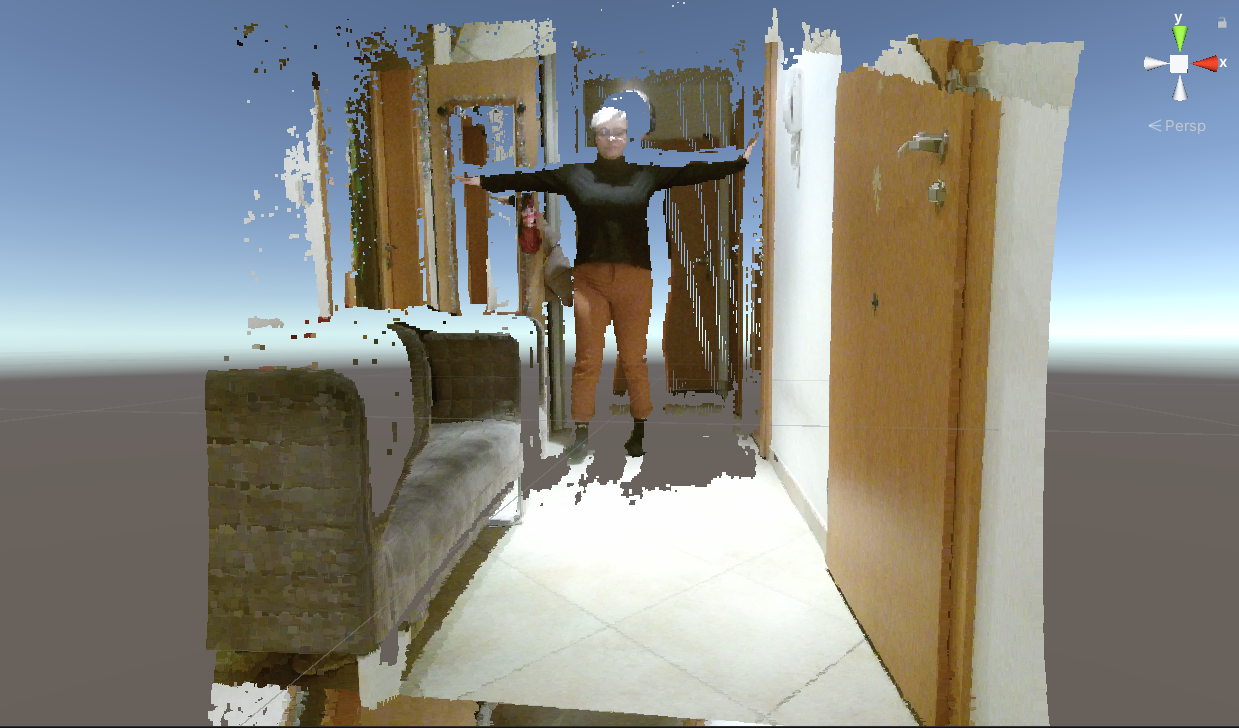
\includegraphics[width=.45\textwidth , keepaspectratio]{images/pointCloud/Screenshot 2021-05-14 211519.png}
\end{subfigure}
\caption{Point cloud density comparison. Left image: small number of points of bigger size; right image: bigger number of points of smaller size}
\label{fig:pc_demo_3}
\end{figure}

 
There is a way that may improve the data visualization quality by using KinectFusion (described in detail in \cite{ARpp} and \cite{IndoorKinect}) and scan the background environment in real time. This technology recreates the environment captured by Kinect cameras using 3D reconstruction of higher quality. This approach has not been implemented in my thesis yet, but it can become a possible future improvement of this application. 




 \bigskip Kinect provides a body index buffer [figure \ref{fig:pc_demo_2}], storing the index of the detected body; if there is no user body in that point, 0 is stored at this point. These data were used to remove the background from the point cloud.

To remove points not related to the user's body, body index texture was used as a stencil. Then, discarding those points where the index value is equal to zero, I have obtained the point cloud without a background [figure \ref{fig:pc_demo_4}].



\begin{figure}[H]
\centering
\begin{subfigure}{\textwidth}
  \centering
  \includegraphics[width=.45\textwidth , keepaspectratio]{images/pointCloud/Screenshot 2021-05-13 174257.png}
\end{subfigure}%
\begin{subfigure}{\textwidth}
  \centering
 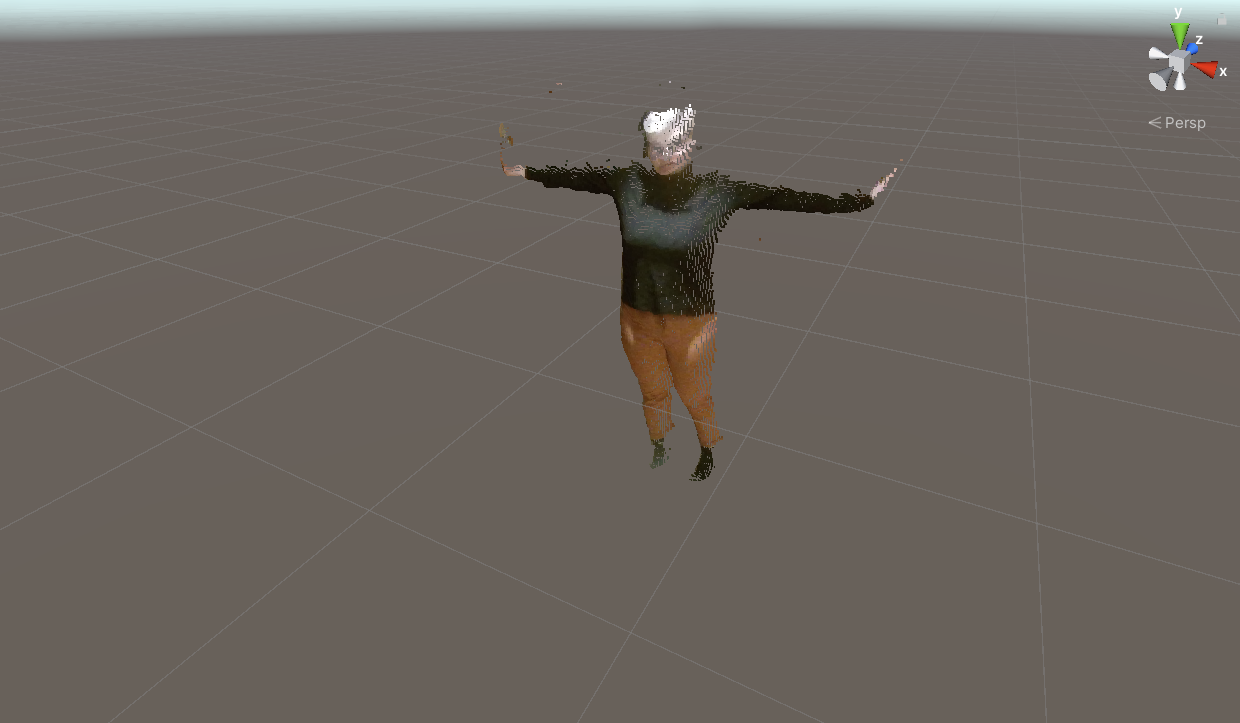
\includegraphics[width=.45\textwidth , keepaspectratio]{images/pointCloud/Screenshot 2021-05-13 174343.png}
\end{subfigure}
\caption{Background removal feature demonstration.}
\label{fig:pc_demo_4}
\end{figure}


This allowed me to create custom backgrounds [figure \ref{fig:backgroungdemo}] using free 3D assets from Unity Asset Store \cite{assetUnity_1}\cite{assetUnity_2}. There are three of them in the application and the user can switch between them easily, these backgrounds are called "rooms" in the application.


\begin{figure}[H]
\centering
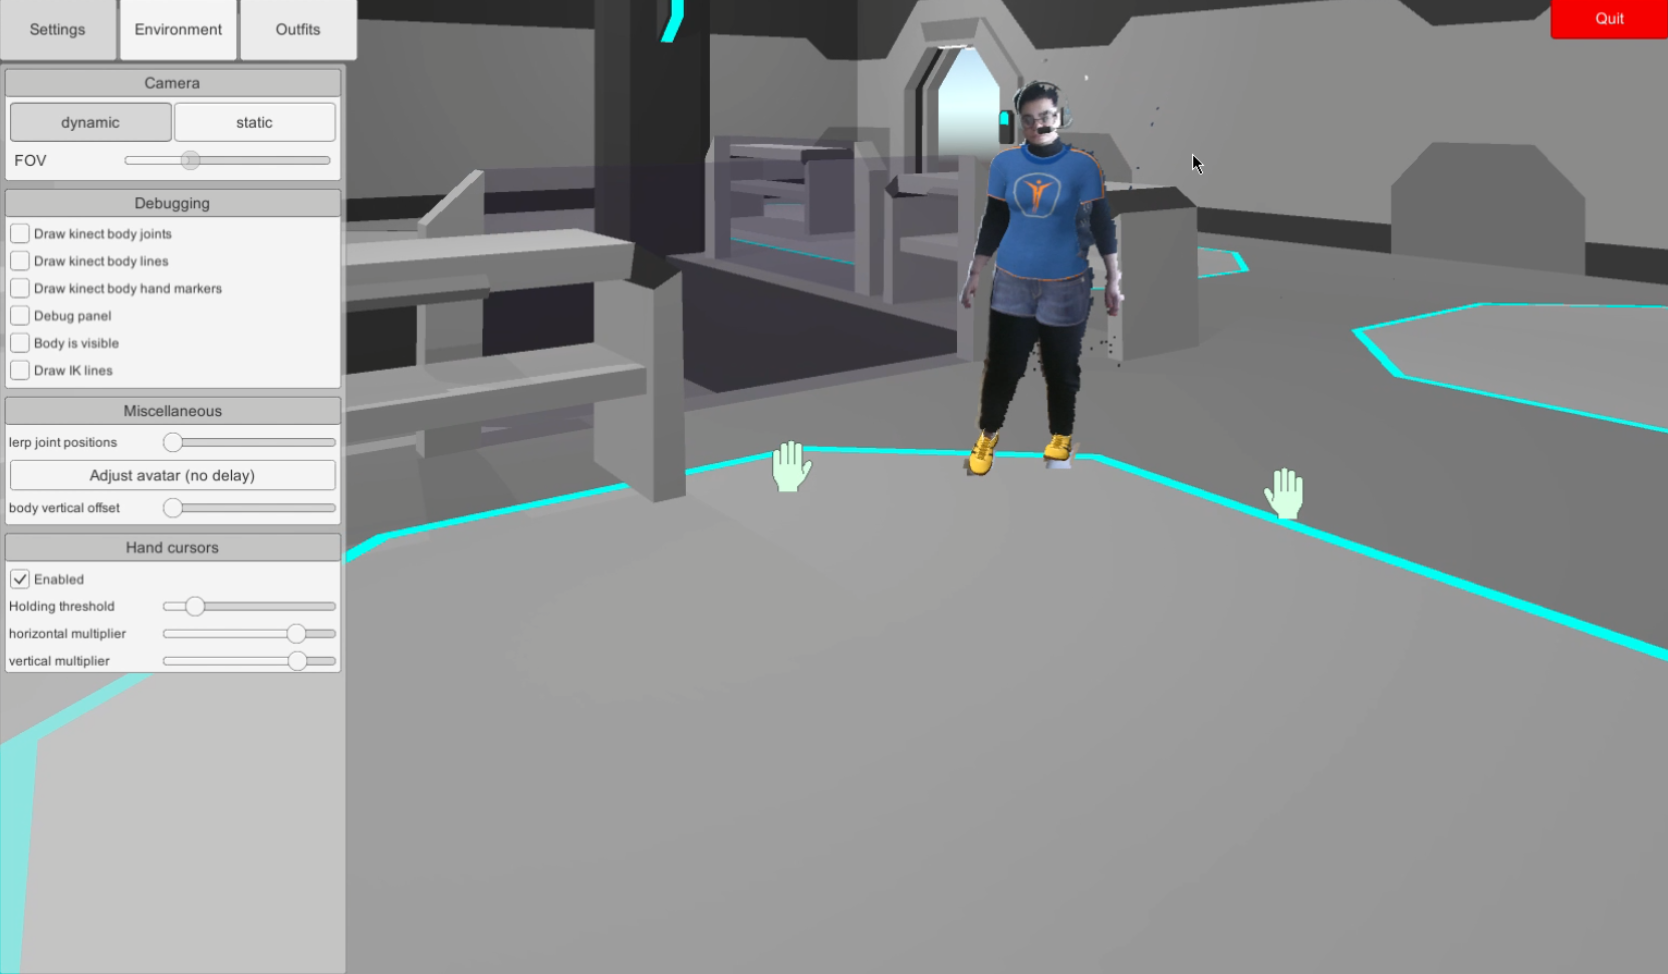
\includegraphics[width=\textwidth , keepaspectratio]{images/OffAxis/off_axis_1.png}
\caption{Point cloud with removed background and 3D meshes in the scene.}
\label{fig:backgroungdemo}
\end{figure}


\section{Inverse Kinematics}
\label{section_avatar}
 \qquad With the help of the Kinect SDK, it was possible to access the position of the detected user and, as a result, the position of his joints. I could add a rigged 3D avatar to the scene and bind the position of its joints to the user's joints, but this leads to distortions of the avatar's geometry [\ref{section_Outfit_visual}]. Due to the differences in the proportions of different parts of the user's body and the skeleton of the avatar, the latter will inevitably be deformed. Worse, due to inaccuracies in capturing the user's movement, the proportions of the Kinect's body are constantly changing by little. This was the reason why I decided to use inverse kinematics for avatar animation [figure \ref{fig:IK_usage}].
 
 
 \begin{figure}[H]
\centering
\begin{subfigure}{\textwidth}
  \centering
  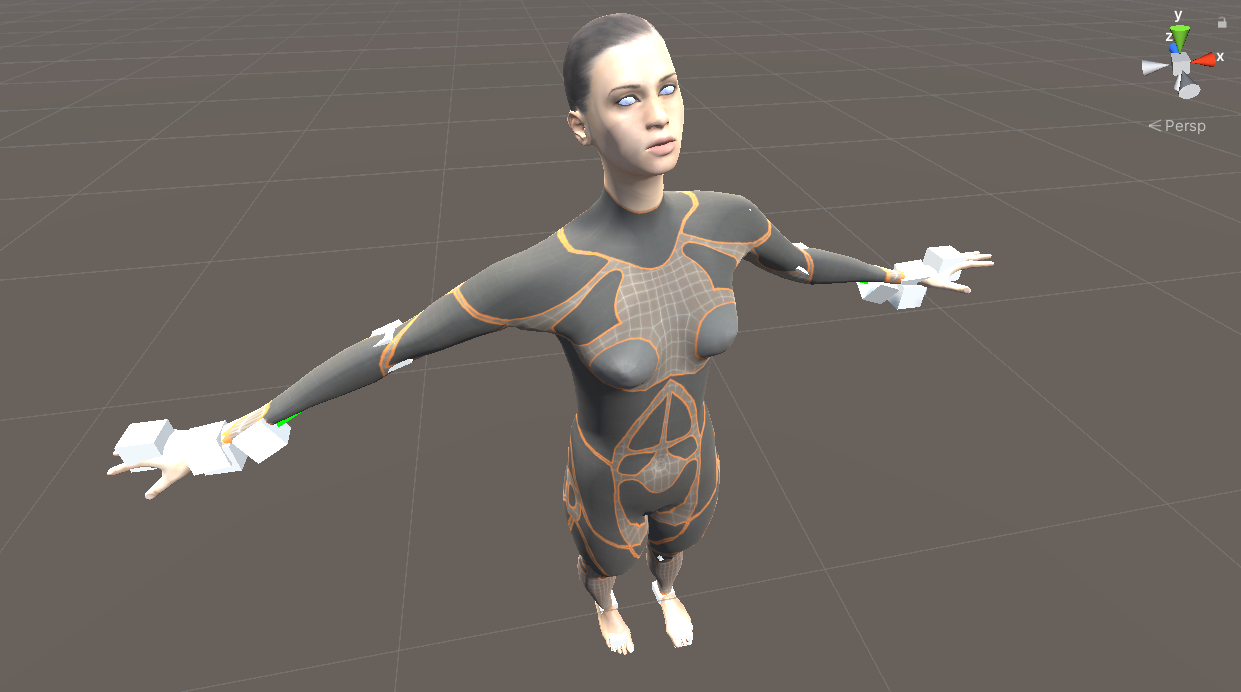
\includegraphics[width=.45\textwidth , keepaspectratio]{images/IK/Screenshot 2021-05-17 093134.png}
\end{subfigure}%
\begin{subfigure}{\textwidth}
  \centering
 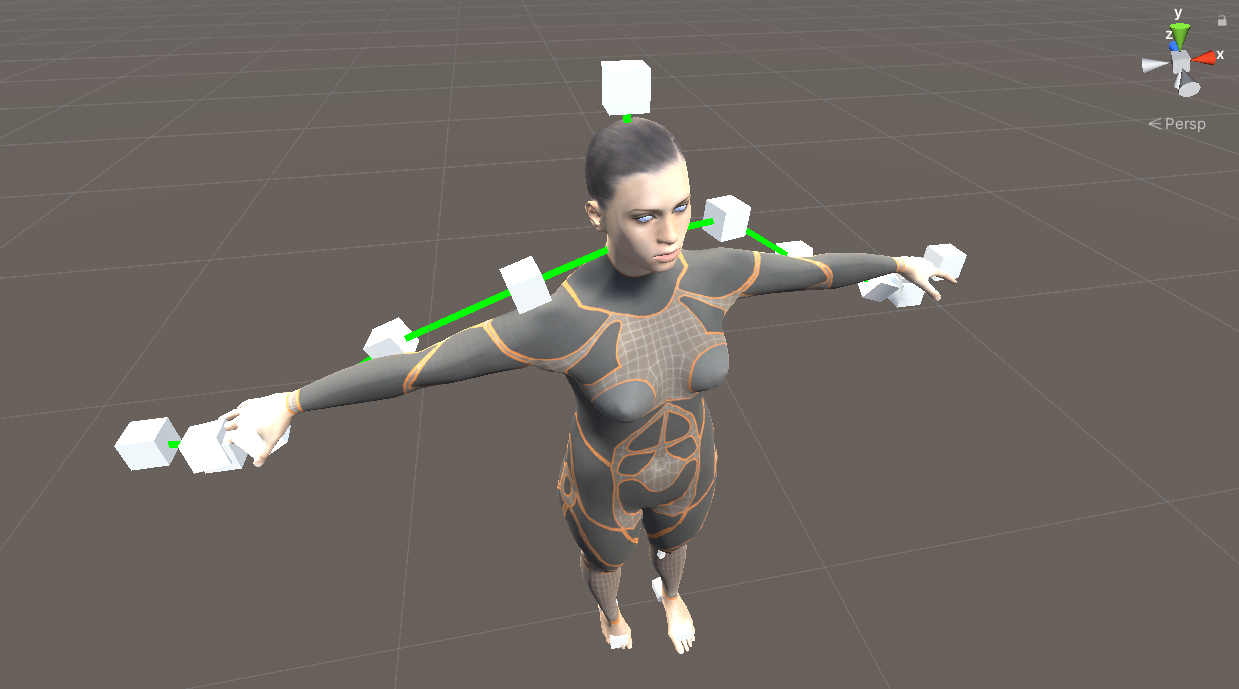
\includegraphics[width=.45\textwidth , keepaspectratio]{images/IK/Screenshot 2021-05-17 093228.png}
\end{subfigure}
\caption{Animation without (left) and with (right) inverse kinematics.}
\label{fig:IK_usage}
\end{figure}
	
 
 
 \subsection{FABRIK Algorithm}
 \qquad In this implementation, it was decided to use the FABRIC algorithm without constraints. The constraints are increasing the execution time of the IK algorithms and there are also problems with deadlock when using the constraints, i.e., a solution is never found because of the constraints\cite{ikmocap}, limiting the chain’s rotation, even though a solution exists. 

 \qquad To describe the mechanics of the inverse kinematics, let us define some terms that are necessary for the following explanation. The point, to which the chain of joints is reaching, is called \textit{the target}. \textit{The end effector} is the last node in the chain which strives to target position. \textit{The hint} is the point where the middle chain node aims.

 \begin{figure}[H]
  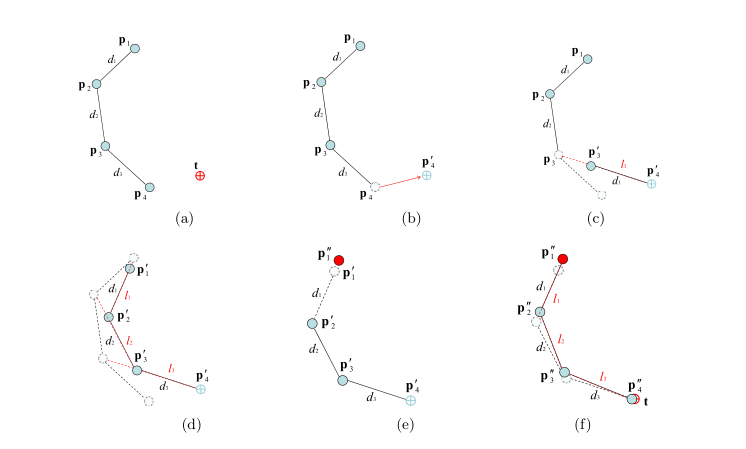
\includegraphics[width=\textwidth, keepaspectratio]{images/Scemas/FABRIK.png}
  \caption{FABRIK algorithm. Image source: \cite{IKtechniques}.} 
  \label{fig:fabrik_alg}
\end{figure}
 
 
\bigskip “An example of a full iteration of FABRIK for the case of a single target and 4 manipulator joints. (a) The initial position of the manipulator and the target, (b) move the end effector p4 to the target, (c) find the joint p′ 3 which lies on the line l3, that passes through the points p′ 4 and p3, and has distance d3 from the joint p′ 4, (d) continue the algorithm for the rest of the joints, (e) the second stage of the algorithm: move the root joint p′ 1 to its initial position, (f) repeat the same procedure but this time start from the base and move outwards to the end effector. The algorithm is repeated until the position of the end effector reaches the target or gets sufficiently close“ \cite{IKtechniques} [figure \ref{fig:fabrik_alg}].

\bigskip I have considered positions of last joints, such as wrists and feet, as targets for limb effectors. In this thesis, I used IK chains to animate legs, arms and spine of the avatar.
Orientation of pelvis and chest was calculated based on position of neighbour joints, as the three joints form a plane, and I could use its normal as a forward direction.
Since the Kinect body data does not contain the orientation of the user's head or any associated joints to calculate it (as it did for the pelvis and the chest), I was forced to use KinectFace plugin. And with its help, to match the rotation of the user's face to the orientation of the avatar's head.

The following image compares my implementation of FABRIK algorithm to default Unity IK [figure \ref{fig:IK_fabrik_vs_unity}].

 \begin{figure}[H]
\centering
\begin{subfigure}{\textwidth}
  \centering
  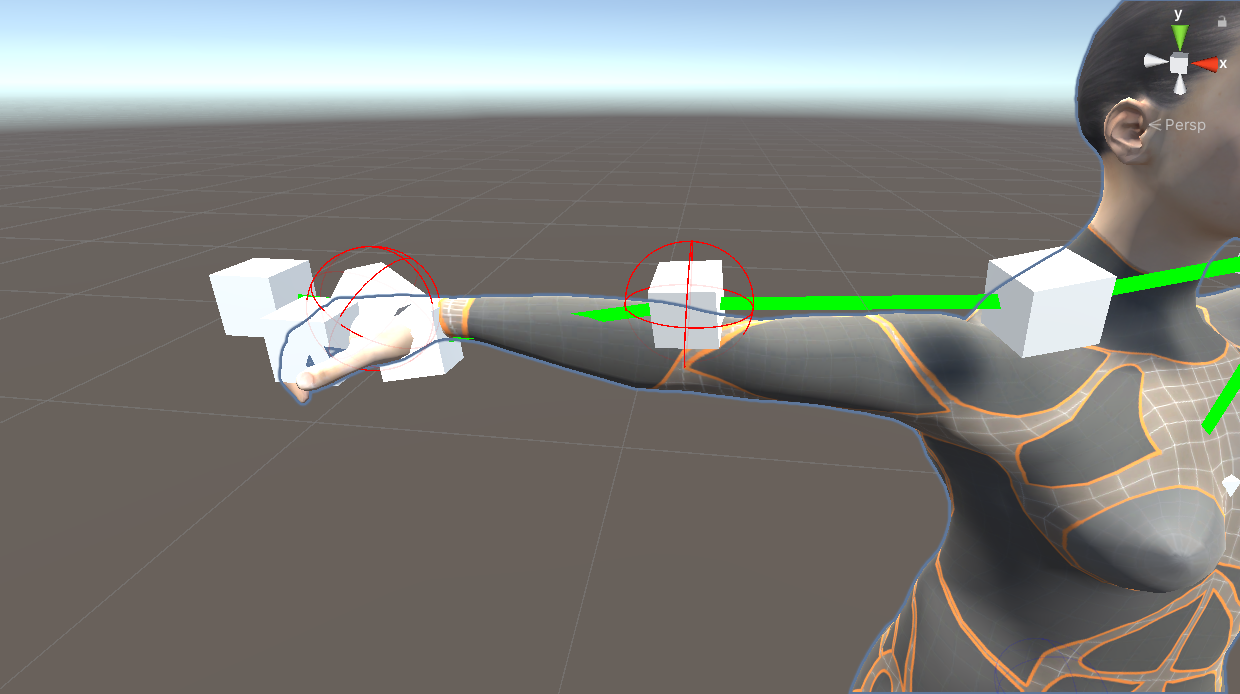
\includegraphics[width=.45\textwidth , keepaspectratio]{images/IK/unity_ik_hand.png}
\end{subfigure}%
\begin{subfigure}{\textwidth}
  \centering
 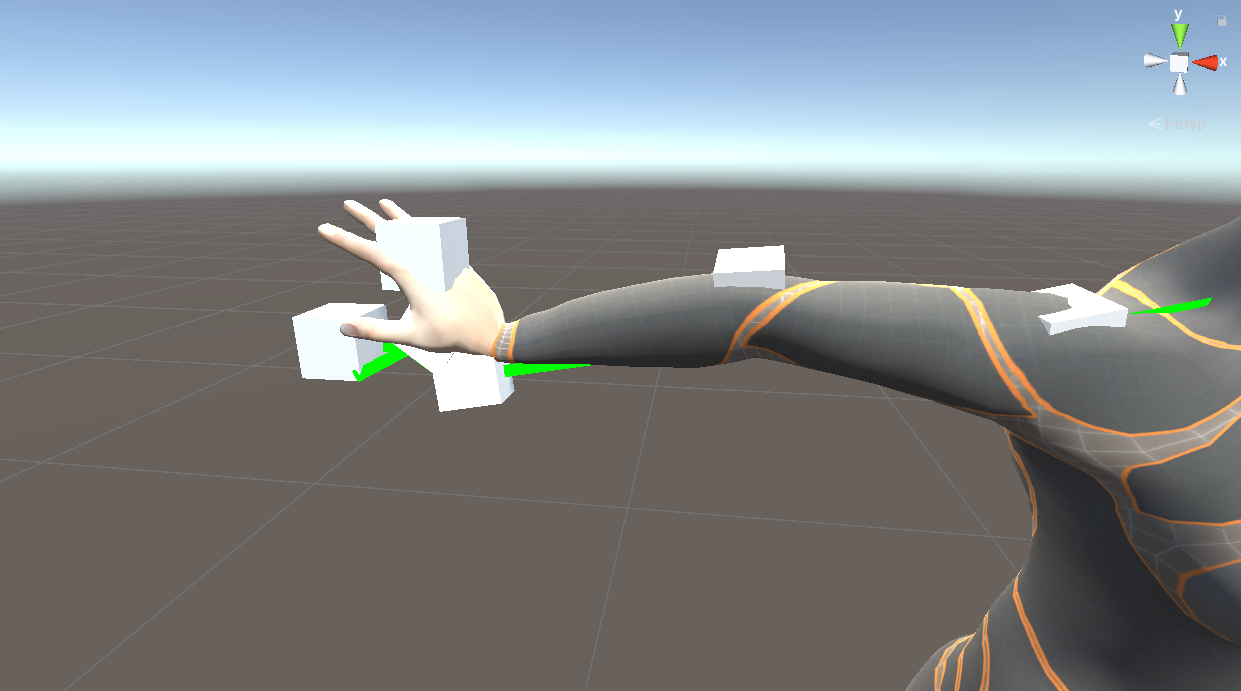
\includegraphics[width=.45\textwidth , keepaspectratio]{images/IK/diy_ik_hand.png}
\end{subfigure}
\caption{Unity inverse kinematics (left) compared to FABRIK (right).}
\label{fig:IK_fabrik_vs_unity}
\end{figure}
	

\bigskip In the future, it is possible to switch to the IK method with multiple end effectors (i.e. turn the torso using the IK branched chain)\cite{upbodyIK}.


\bigspace By applying FABRIK I have achieved the proper animation of the avatar based on the user's movements.


\section{Outfit Rendering}

\qquad When rendering clothes, it was necessary to take into account that the outfits had to be displayed on top of the user's image [figure \ref{fig:rendering_clothes_order_1}]. Additionally, I had to hide the parts of the clothes that are not visible in reality; for example the insides of the clothes are covered by the person wearing them and are not seen in real life. 

\subsection{Rendering order} 

\qquad Point cloud and avatar with clothes meshes are placed on different render layers. Thus, the avatar and the clothes meshes are always rendered on top of the point cloud, each layer is rendered with its own camera separately [figure \ref{fig:rendering_clothes_order_2}].

 \begin{figure}[H]
  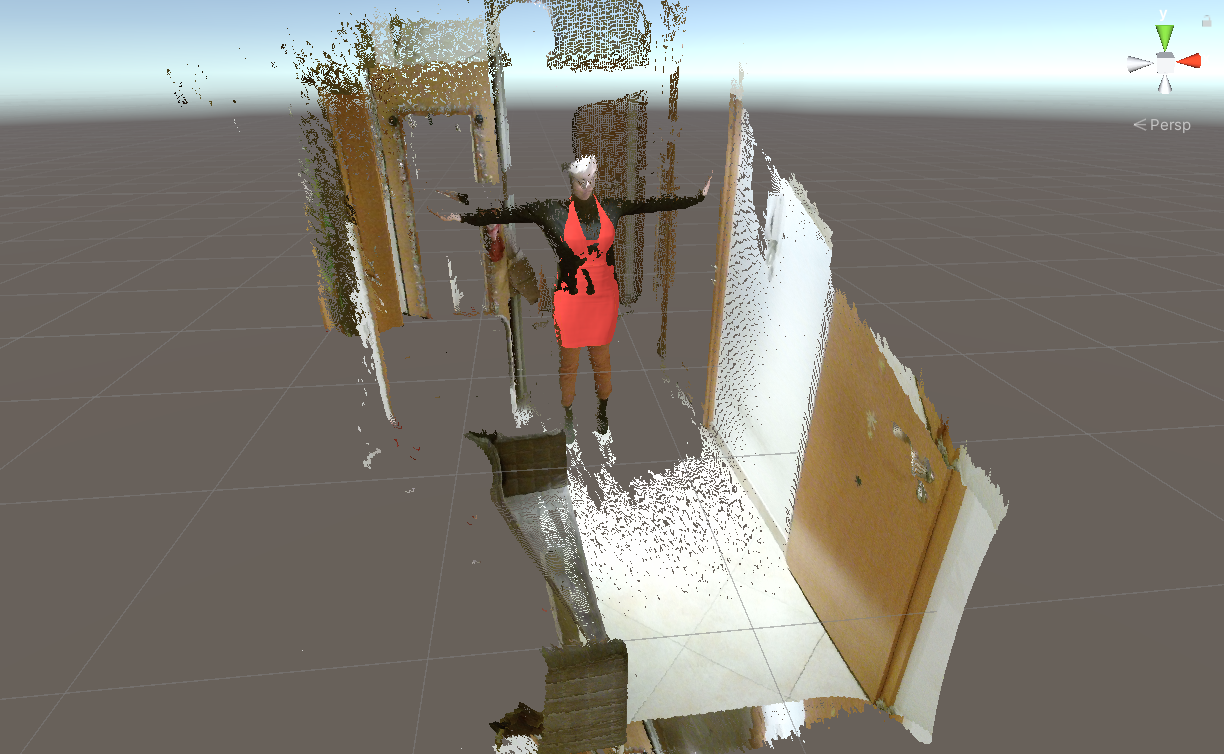
\includegraphics[width=\textwidth, keepaspectratio]{images/ClothesDemos/Screenshot 2021-05-14 190249.png}
  \caption{ Outfit and the point cloud rendered on the same layer.} 
  \label{fig:rendering_clothes_order_1}
\end{figure}





 \begin{figure}[H]
    
  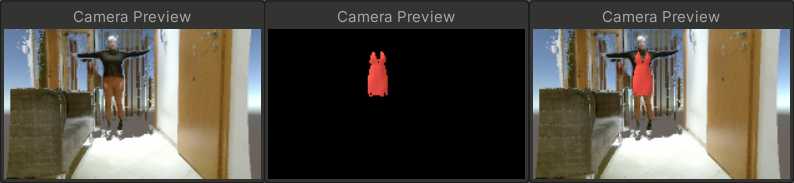
\includegraphics[width=\textwidth, keepaspectratio]{images/ClothesDemos/render_layers_1.png}
  \caption{Different layers rendering. The last image is the result of combination of the previous two images.} 
  \label{fig:rendering_clothes_order_2}
\end{figure}




\subsection{Usage of stencil buffer for outfits rendering}
\qquad During clothes rendering the following issue occurred: when we draw a mesh of clothes on an invisible body, those parts that are closed by the body should not be visible.


 \begin{figure}[H]
    \begin{subfigure}{\textwidth}
  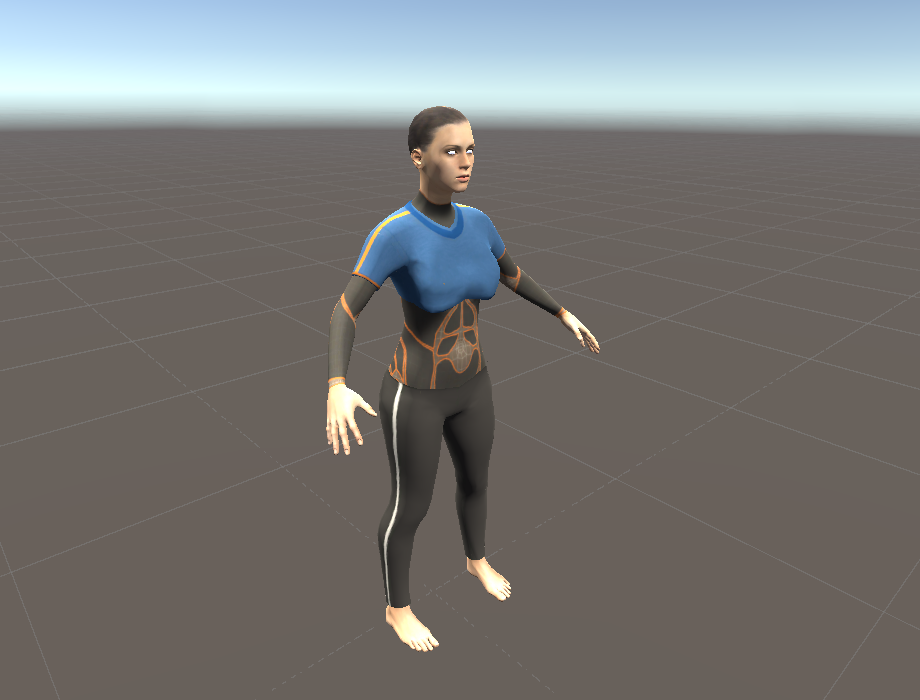
\includegraphics[width=.465\textwidth, keepaspectratio]{images/ClothesDemos/normal_meshes.png}
   \end{subfigure}%
    \begin{subfigure}{\textwidth}
  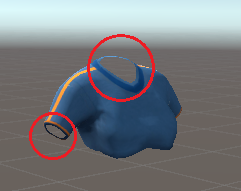
\includegraphics[width=.45\textwidth, keepaspectratio]{images/ClothesDemos/normal_outfit_mesh_with_arrows.png}
   \end{subfigure}%
  \caption{Clothes visualization issue.} 
  \label{fig:stencil_err_1}
\end{figure}

At first glance, it seems I could rely on face culling, which imposes additional requirements on the geometry of the model. However, as you can see in the picture on right, there are triangles (faces) turned towards the camera, that must not be rendered, because they are positioned behind the “invisible” body.

The solution I came out with was to use the stencil buffer to set the correct stencil for rendering.
To do this, I had to implement three different shaders, each for its own step.

The green color on the following pictures show the values of the stencil buffer after shader execution.



\textbf{1. Rendering the clothes mesh with shader\_1.}
\begin{itemize}
    \item Stencil buffer is filled for the whole mesh;
    \item Mesh rendering is done in transparent color and writing to the depth buffer is enabled.
\end{itemize}

 \begin{figure}[H]
  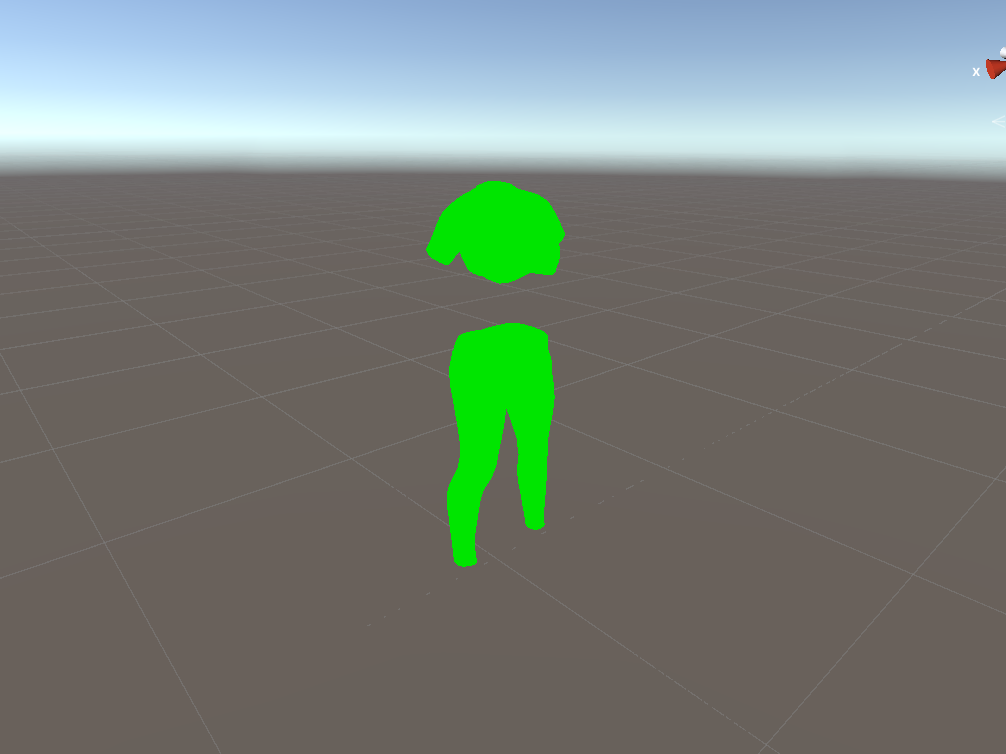
\includegraphics[width=\textwidth, keepaspectratio]{images/ClothesDemos/Screenshot 2021-05-08 175145.png}
  \caption{stencil buffer values after execution of shader\_1.} 
  \label{fig:stencil_sh_1}
\end{figure}


\textbf{2. Rendering the clothes mesh with shader\_2.}

\begin{itemize}
    \item The current values of the stencil buffer are used as a stencil to prevent doing beyond its scope;
    \item Where the depth check passes (the body is closer to the camera than the mesh vertex), the stencil buffer value is set to 0;
    \item Writing to the depth buffer is disabled, because we do not want other objects in the scene to be overwritten with the “transparent background color” of the body.
\end{itemize}

 \begin{figure}[H]
  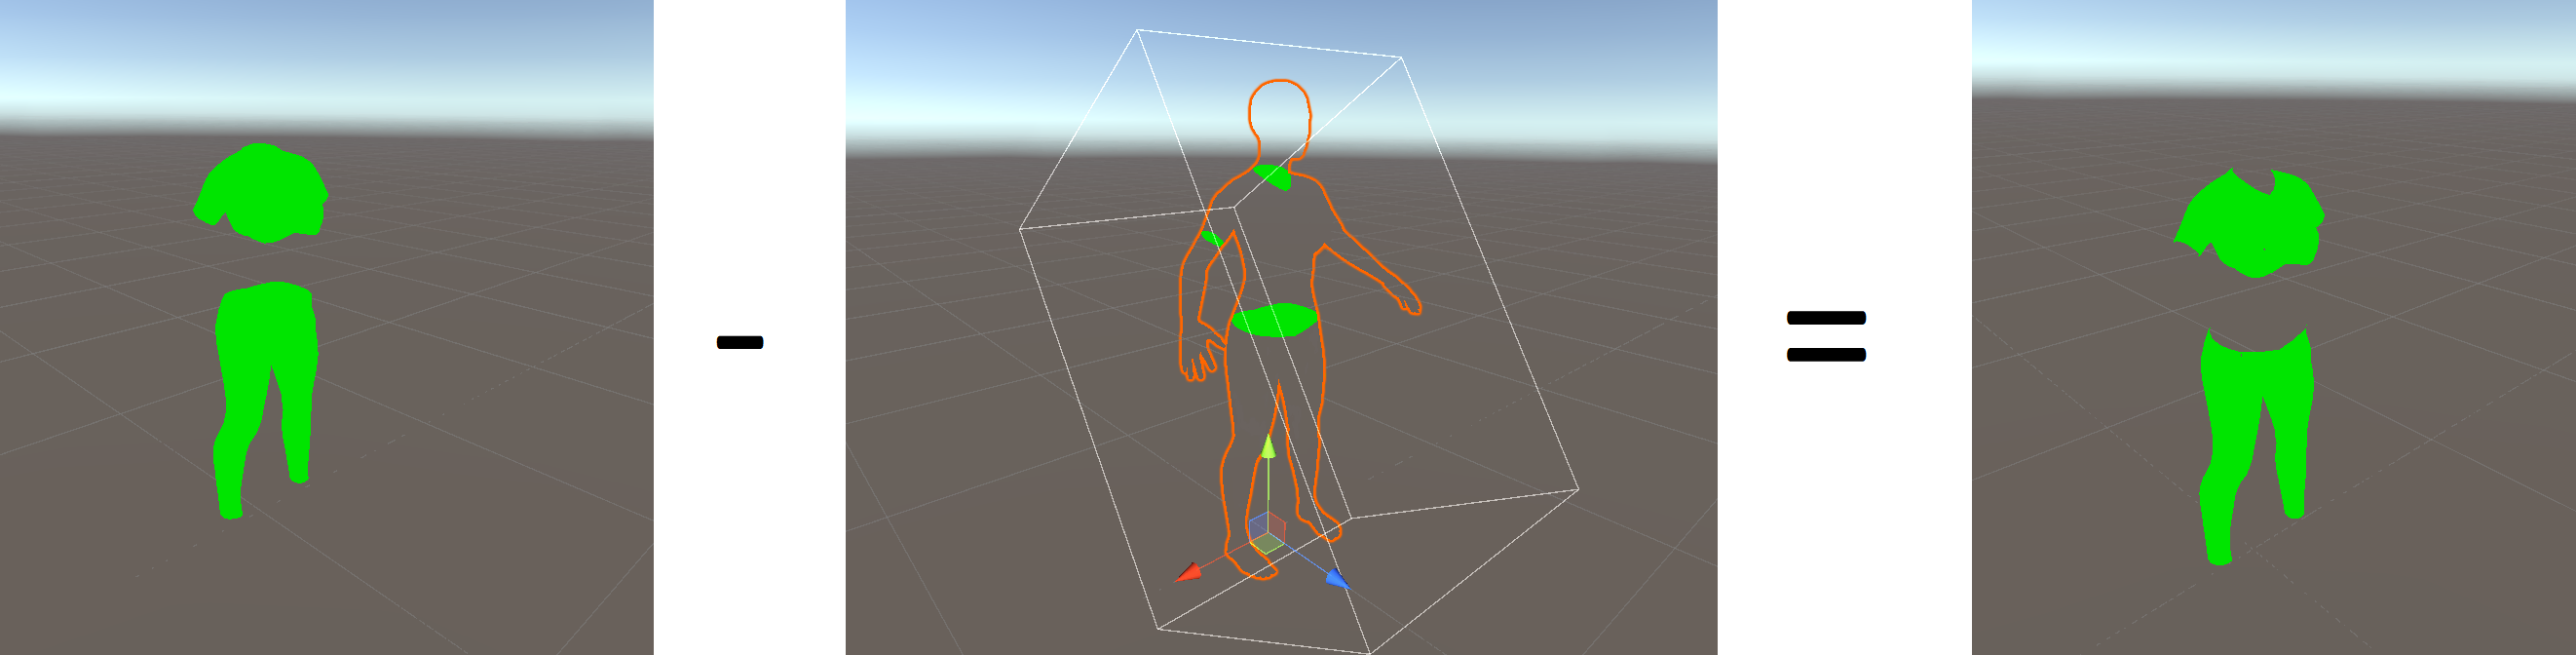
\includegraphics[width=\textwidth, keepaspectratio]{images/ClothesDemos/3_outfit_-_cutted_body_result_new.png}
  \caption{The final picture on the right represents the stencil buffer values after execution of shader\_2. The image in the center is placed here only for demonstration purposes, such buffer state never exists in the implementation.} 
  \label{fig:stencil_sh_1}
\end{figure}




\textbf{3. Rendering the clothes mesh with shader\_3.}

\begin{itemize}
    \item Normal rendering using stencil buffer values.
\end{itemize}

\textbf{Final result:} only the "visible" parts of the mesh are drawn. 


 \begin{figure}[H]
  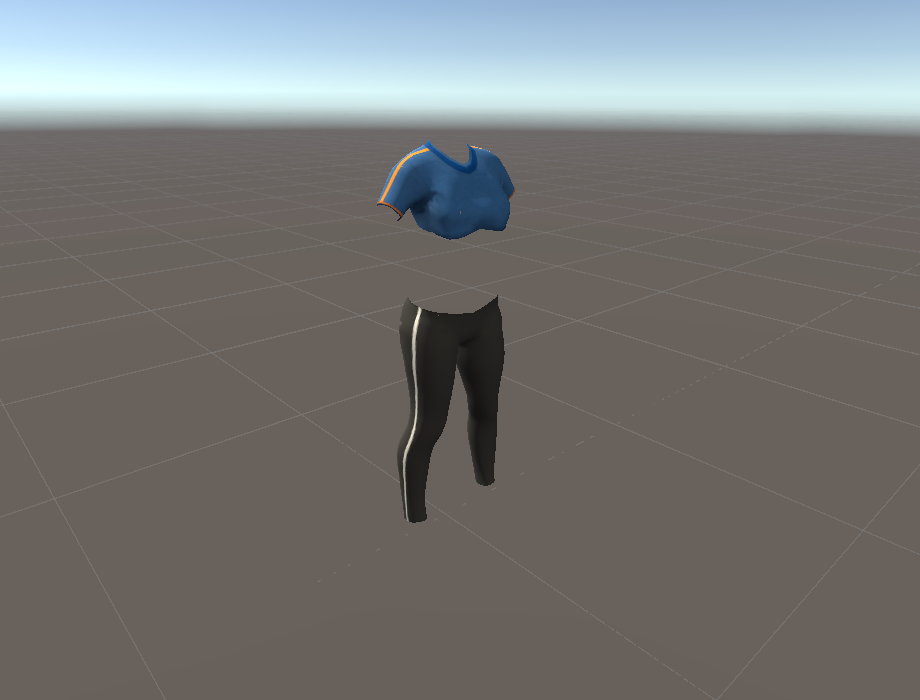
\includegraphics[width=\textwidth, keepaspectratio]{images/ClothesDemos/4_render_outfit_using_result_stencil.png.png.png}
  \caption{The outfit mesh rendered using stencil buffer.} 
  \label{fig:stencil_sh_1}
\end{figure}



\subsection{Avatar Attunement} 
\qquad Due to the variety of human bodies there is no way to prepare a universal avatar which will fit any user. Thus some kind of an attunement is required:

\begin{itemize}
    \item in terms of height and constitution the simplest approach is just to scale the avatar;
    \item next step is stretching avatar bones to match the lengths of users limbs;
\end{itemize}

These avatar settings were implemented in the project; the scaling option and the bones stretching is computed in the application based on the user's joints positions.




\section{Clothing Combination System}
\label{section_clothes_combo_system}

\qquad To fulfill the thesis task I had to implement a system, that would allow users to combine clothing pieces from different categories and try them on all together at the same time. This led to the following problems:

\begin{itemize}
    \item the ability to wear one item of clothing over another (e.g. a jacket over a shirt);
    \item the body of the avatar should not be visible through clothing;
    \item clothes of the bottom layer should not be visible through the clothes of the top layer.
\end{itemize}

To generate different types of bodies and clothes for them, the Makehuman program was used. Furthermore, I used clothing models available for free use as well.


It was decided to divide all possible clothes into the following categories [figure \ref{fig:clothesIcons}]:
\begin{itemize}
    \item hats
    \item gloves
    \item tops - lower layer
    \item bottoms - lower layer
    \item tops - upper layer
    \item bottoms - upper layer
    \item shoes
\end{itemize}


 \begin{figure}[H]
  
\includegraphics[width=\textwidth, keepaspectratio]{images/ClothesCombination/category_buttons.png}
  \caption{Clothes categories icons used in the application, icons sources: \cite{iconCap}\cite{iconGLoves}\cite{iconUndershirt}\cite{iconUnderwear}\cite{iconJacket}\cite{iconJeans}\cite{iconShoe}
  } 
  \label{fig:clothesIcons}
\end{figure}


In this case, a particular piece of clothing can occupy several slots (categories) at once, for example, a business suit includes a shirt ( a top, lower layer), a jacket (a top, upper layer) and trousers (a bottom, upper layer).

Thus, if the avatar is already wearing gloves, jeans and boots, and the user would like to to wear a business suit, then the jeans will be removed. As a result, the avatar will be equipped with gloves, boots and a business suit.



\subsection{Clothes Layering}

\qquad When the avatar moves, the body mesh may go through the mesh of the clothing, even if in the T-pose the clothing covered the body flawlessly without intersections. The MakeHuman application implements the removal of body faces in those places that are covered by clothes and should not be visible [figure \ref{fig:bodymesh_edit}].
For this thesis, I relied on meshes generated in MakeHuman and used this feature.

\begin{figure}[H]
\centering
    \begin{subfigure}{\textwidth}
      \centering
      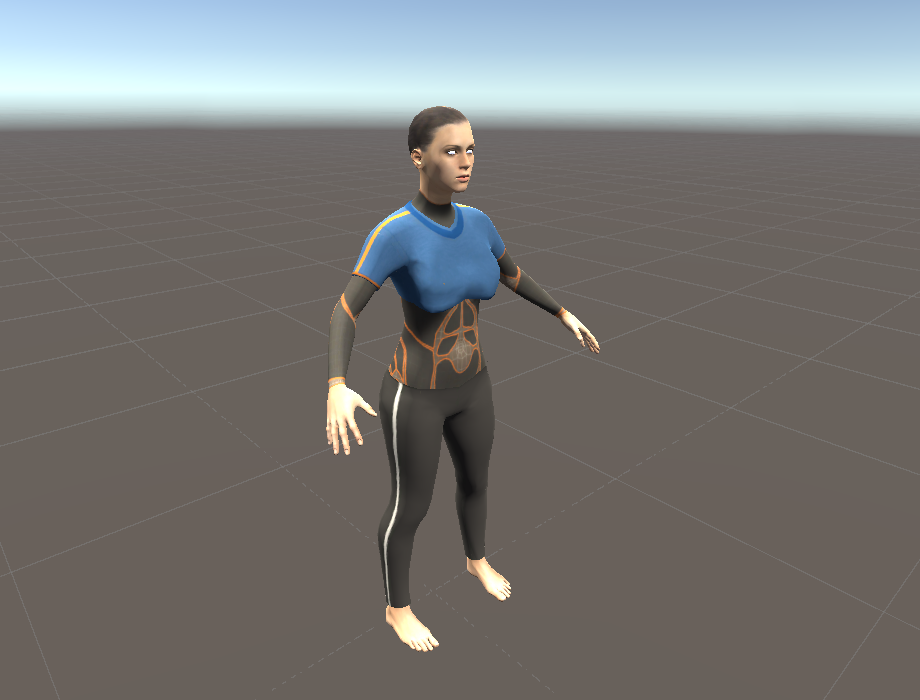
\includegraphics[width=.45\textwidth , keepaspectratio]{images/ClothesDemos/normal_meshes.png}
    \end{subfigure}%
    \begin{subfigure}{\textwidth}
      \centering
      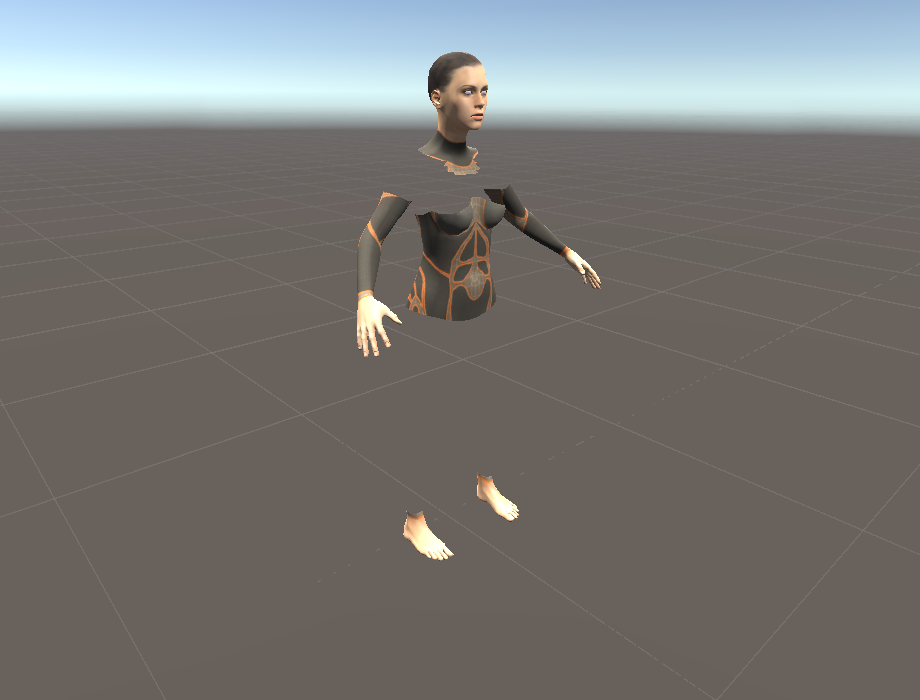
\includegraphics[width=.45\textwidth , keepaspectratio]{images/ClothesDemos/normal_body_mesh_some_faces_cut.png.png.png}
    \end{subfigure}
\caption{MakeHuman editing the body mesh.}
\label{fig:bodymesh_edit}
\end{figure}
 
Next, I had to solve the problem of layering clothes pieces on top of other clothes pieces, for example, combining two different objects: a shirt and a jacket, and prevent the 3D models from intersecting during animation. In general, the problem is complex and there is no universal approach for real-time applications \cite{layeredClothing}.

The easiest way to make sure that different layers of clothing do not conflict with each other is to manually prepare a new mesh for each combination of clothing. Obviously, the number of combinations is rapidly increasing with the increase of the number of clothing items. For the purposes of the thesis, it was decided to prepare only combinations of  (eg. shirts and jackets) for each of the body types. For $n$ items of lower layer tops and $m$ items of upper layer tops it is only $n*m$ combinations. 

This approach is implemented in the following way:  after the user picks an item of clothing, a search is made among the prepared combinations.
Thus, if the avatar is wearing, for example, jeans, a shirt and a jacket, and there is a prepared combination of these jacket and the shirt, the standalone objects of the jacket and the shirt will be replaced with the premade combination, and the jeans will remain intact.









\subsection{Clothing layering using stencil buffer}

\qquad Each piece of clothing requires its own body mesh to correctly remove the parts that should not be visible. However, if several items of clothing are presented at the same time and, accordingly, several bodies, then faces removed from one body are replaced by faces from another body [figure \ref{fig:stenc_1}].

\begin{figure}[H]
\centering
    \begin{subfigure}{\textwidth}
      \centering
      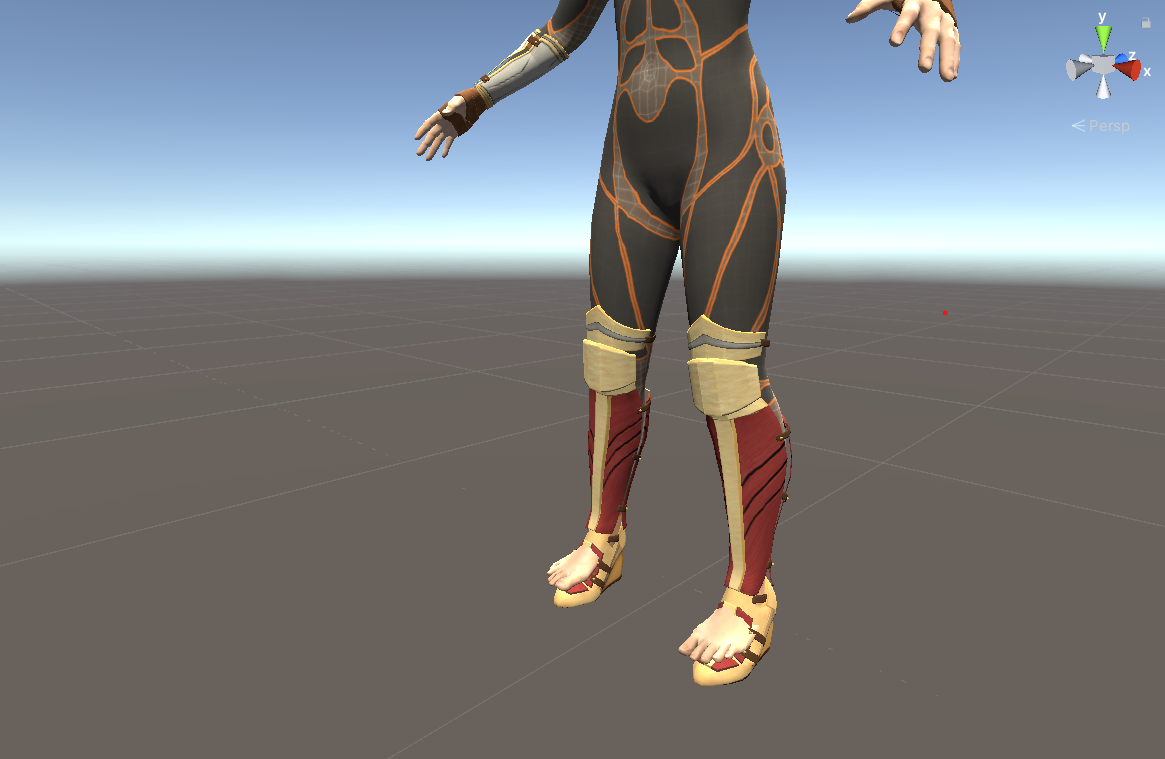
\includegraphics[width=.45\textwidth , keepaspectratio]{images/ClothesDemos/Screenshot 2021-05-08 215039.png}
    \end{subfigure}%
    \begin{subfigure}{\textwidth}
      \centering
      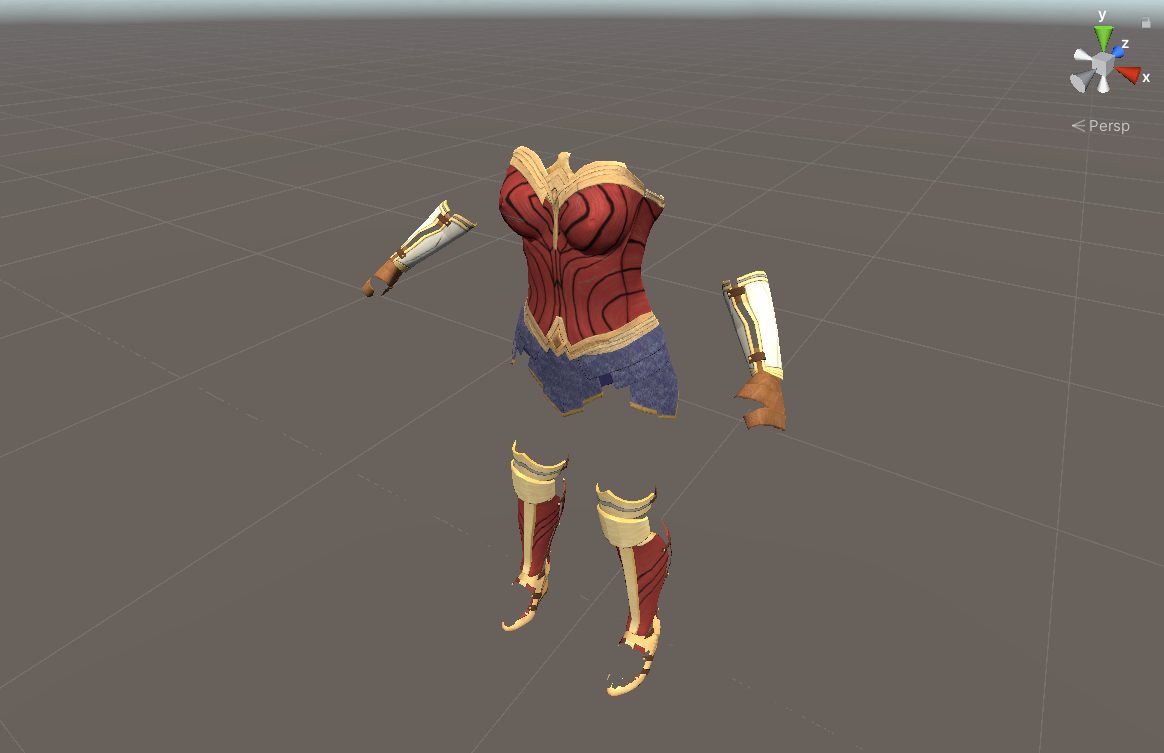
\includegraphics[width=.45\textwidth , keepaspectratio]{images/ClothesDemos/Screenshot 2021-05-08 221538.png}
    \end{subfigure}
\caption{The toes are parts of the body provided by the piece of clothing other than the boots. This causes "holes" in the outfit.}
\label{fig:stenc_1}
\end{figure}

To solve this issue, I have decided to store the category for each clothing piece in the form of flags. Thus, if the flag in binary representation 00000001 encrypts the top of the outerwear, 00000010 encrypts the top of the underwear, and 00000100 encrypts the bottom of the outerwear, then the business suit should have the category 00000111 [figure \ref{fig:stenc_2}].

\begin{figure}[H]

    \centering
    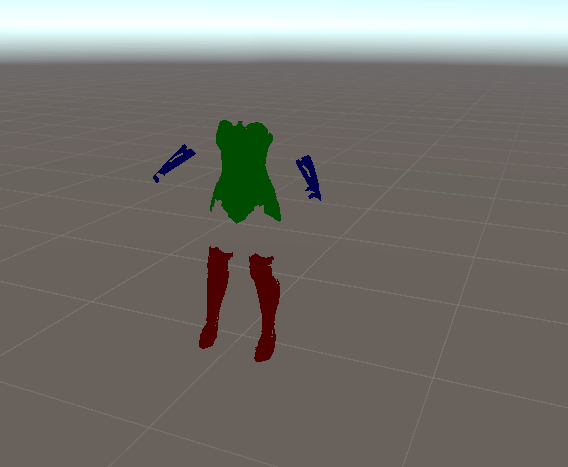
\includegraphics[width=\textwidth , keepaspectratio]{images/ClothesDemos/Screenshot 2021-05-08 215143.png}
    \caption{Demonstration of the stencil buffer after rendering each piece of clothing. Colors represent the state of the stencil buffer.}
    \label{fig:stenc_2}
\end{figure}

Since the stencil buffer allows bitwise reading and writing using a bit mask, I have used the bit representation of the clothing category as such. The stencil buffer cell size is 8 bits, which is enough for the needs of this work, since only 7 categories are used here. This approach allowed me to consider each bit of the stencil buffer individually and operate on the visibility of meshes of different clothing items independently of each other [figure \ref{fig:stenc_3}].


\begin{figure}[H]
    \centering
    \includegraphics[width=\textwidth , keepaspectratio]{images/ClothesDemos/Screenshot 2021-05-08 221401.png}
      
    \caption{The correct result of combination.}
    \label{fig:stenc_3}
\end{figure}


\subsection{Outfit Models}
\label{section_models}
\qquad Most of the assets for this implementation were taken from MakeHuman application \cite{makehuman}, that allows exporting human bodies and clothes [figure \ref{fig:makehuman_outfit}] and using them in non-commercial projects, some of the clothes assets were taken from MakeHuman community page \cite{makehumanCommunity}. 

These assets were used in the application for demonstration purposes, as I was not able to get access to any kind of historical clothing, that was recreated in 3D form using photogrammetry. However, the used 3D models could be replaced with the proper 3D reconstructed ones to make the application usable in the museum environment.



\begin{figure}[H]
\centering
  \includegraphics[width=\textwidth, keepaspectratio]{images/Models/model_makehuman.png}
  \caption{Example of an outfit from MakeHuman.}
  \label{fig:makehuman_outfit}
\end{figure}






\section{User Interface}
\label{section_ui}

\qquad At first, it was decided to implement a simple UI that is controlled by a mouse, all the panels, buttons and checkboxes were implemented using standard Unity User Interface design tools.  

%===== NEW UI =======

The UI consists of three main tabs:

\begin{itemize}
    \item The Settings tab [figure \ref{fig:ui_1}] contains the camera settings (static camera with on-axis projection / dynamic camera with off-axis projection and a Field of view slider), debugging tools and hand cursors settings, that will be used for interactions with gestures.
    \begin{figure}[H]
    \centering
    \includegraphics[width=\textwidth, keepaspectratio]{images/UI/UI_1.png}
    \caption{Settings tab demonstration.}
    \label{fig:ui_1}
    \end{figure}
    
    
    \item The Environment tab [figure \ref{fig:ui_2}] allows switching from 2D view to the Point cloud representation and contains Point cloud settings (the remove background feature and the background(room) selection feature).
    \begin{figure}[H]
    \centering
    \includegraphics[width=\textwidth, keepaspectratio]{images/UI/UI_2.png}
    \caption{Environment tab demonstration.}
    \label{fig:ui_2}
    \end{figure}
    
    
    \item The Outfits tab [figure \ref{fig:ui_3}] contains the avatar picking and adjusting features and the selection of clothing available for each avatar individually. 
 
    \begin{figure}[H]
    \centering
    \includegraphics[width=\textwidth, keepaspectratio]{images/UI/UI_3.png}
    \caption{Outfits tab demonstration.}
    \label{fig:ui_3}
    \end{figure}

\end{itemize}



%===== OLD UI =======
%\begin{figure}[H]
%\centering
%  \includegraphics[width=\textwidth, keepaspectratio]{images/UI/UI.pdf}
%  \caption{User Interface explanation.}
%  \label{fig:ui}
%\end{figure}

\subsection{Interactions  With Gestures}

\qquad Even though the implementation of this feature is basic and simple, it can be used as an additional way of interaction.

There are 2 pseudo cursors in the scene, one for each palm. The hand position is translated into screen coordinate space, then applied to the cursor. The state of the palm (open or closed) is interpreted as pressing the left mouse button [figure \ref{fig:gestures}].

While implementing such an approach I have faced the following issues:

\begin{itemize}
\item The palm state is best detected closer to the center of the screen.
\item Frequent false detection of closing the palm and low accuracy in determining the state of the palm in general.
\end{itemize}

I have solved them with the following ideas:

\begin{itemize}
\item The cursor position is dynamically shifted due to multiplication of the cursor's coordinate by a constant. Thus, the user could, being in the middle of the Kinect's field of view, reach with the cursor to the edges of the screen and interact with the interface elements.
\item While the hand is continuously defined as closed, the time spent in the closed position is accumulated. If this time is more than a certain value, then left mouse button (LMB) pressing is emulated. If the hand was open before the threshold value was reached, then no clicking occurs, and the time recorded is reset.
\end{itemize}

\begin{figure}[H]
    \begin{figure}[H]
    \centering
    \includegraphics[width=\textwidth, keepaspectratio]{images/UI/gestures_1.png}
    \label{fig:gestures_1}
    \end{figure}
    
    \begin{figure}[H]
    \centering
    \includegraphics[width=\textwidth, keepaspectratio]{images/UI/gestures_2.png}
    \label{fig:gestures_2}
    \end{figure}
    
    \caption{Gestures interactions demonstration.}
    \label{fig:gestures}
\end{figure}




\section{Playground room}

\qquad To make the application usage more entertaining, I have decided to add a special room called the Playground [figure \ref{fig:playgroundRoom}], where the user could interact with 3D objects. 

\begin{figure}[H]
\centering
  \includegraphics[width=\textwidth, keepaspectratio]{images/Testing/Screenshot (3).png}
  
  \caption{Playground room.}
  \label{fig:playgroundRoom}
\end{figure}

Currently there are two types of interactions available:
\begin{itemize}
    \item If the user puts his palm inside the yellow cuboid, then random 3D primitives will start spawning in the scene until the user removes his hand.
    \item The user can grab any 3D object in the scene (except for the yellow cuboid) and move it around the space.
\end{itemize}

This specific room combines the possibilities of a virtual fitting room and an interactive game, allowing the users play it while wearing a virtual outfit.

% ================================================================================================%
% ================================== CHAPTER 5 ===================================================%
% ================================================================================================%
\chapter{Application Testing}
\label{chapter_Testing}

\qquad This chapter presents the results of the testing with people and an analysis of a technical side and performance of the application. 

\section{User testing}
    \qquad The application was widely tested by people with variant constitutions, the diversity of the testing grouphttps://www.overleaf.com/project/5ff94e9afb401413537be28c allowed me to analyze the down sides of the implementation and reveal the bugs, that were were not detected during the development process. 
    
    The users were asked to complete the following tasks: 

  \begin{mdframed}
  \bigskip
       \begin{enumerate}
         \item Stand in front of the monitor, look at your mirrored image on the display. You have to see your body fully from head to toes. 
        
         \item Navigate to the Outfits tab using a computer mouse. Choose a preferable body type and adjust it to match your own body by clicking the Adjust Body button.
         
         \item Select one piece of clothing from each category:
         \begin{enumerate}
            \item top - lower layer
            \item top - upper layer
            \item bottom 
            \item shoes
            \item hat
            \item gloves
         \end{enumerate}
     
        
        \item Try moving around the room and/or posing. 
        
        \item Swap selected parts of clothing with any other ones that are available in the menu. 
        
        \item Try picking clothes with gestures. To do so, navigate to the preferred piece of clothing with a hand cursor and make a fist to click. 
        
        \item Either with a computer mouse or with a hand cursor navigate to the Settings tab. You may want to adjust hand cursors positions in the bottom section of the Settings tab. 
        
        \item Either with a computer mouse or with a hand cursor navigate to the Environment tab.
        Change Kinect Visualization type to Point cloud. 
        
        \item Using a PC mouse adjust points size and/or density to your liking. 
        
        \item Click on Remove Background check box and select the Futuristic #1 room. Navigate to the Outfits tab again and pick some clothes. Try to move around the area and/or pose. 
        
        \item Navigate back to the Environment tab and select the Futuristic #2 room. Repeat the try-on experience from the previous step. 
        
        \item Navigate to the Settings tab and select dynamic camera. Keep in mind that the gestures are not working in dynamic camera mode. 
            \begin{enumerate}
                \item Walk around the room to see, if this effect reminds you of the way mirror reflection works.
                \item Using a PC mouse navigate to clothes selection once more, pick some clothes.
                \item Navigate to the Settings tab and switch camera back to static. 
            \end{enumerate}
              
        \item Navigate to the Environment tab and select the Playground room. 
            \begin{enumerate}
                \item Put your right palm inside the big yellow object. This should spawn some random 3d primitives to the scene. 
                \item Try to grab a 3d object with your hand. 
             \end{enumerate}
        
        \item You have now completed the test. To close the application, click on the Quit button. 
        
        \item Please share your thoughts on the application, give some criticism and suggest possible improvements.
        
       \end{enumerate}
        \bigskip
|{
6
[p\end{mdframed}
    
    Although the given tasks were meant to be completed in 30 minutes, most of the users have successfully finished them in lesser time with no hurry. The following sections are dedicated to each tester to summarize their experience with the program. 
      
      

    \newpage
    \subsection{User \#1}
    General personal information:
    \begin{itemize}[label={}]
        \setlength\itemsep{0.025em}
        \begin{AutoMultiColItemize}
            \item Gender: Female
            \item Age Group: 20-25
            \item Height: 156 cm
            \item Clothes size: M
        \end{AutoMultiColItemize}
    \end{itemize}
   
    The user had difficulties with navigation in the application, she did not approve the UI layout, saying that it is not intuitive for a general user. She needed guidance during the testing process to complete the given tasks. The User \#1 was frustrated with the clothes filtering system, she was also complaining about the precision on the body adjustment feature. According to this user, the selection of clothes in the current version is limited and the materials of the clothes are not obvious.

    
    \textbf{Bugs and errors:} 
    due to the user's height there were issues with the automatic body adjustment feature, the body was not scaling correctly and was shifted downwards. The problem was fixed right after this particular test.
    
    \textbf{User’s suggestions on future development:} 
    the user would like to be able to manipulate with clothes, for example, to tuck in a t-shirt or any other top. On practice, that would mean adding physics for the fabric. The tester also suggested a feature to render user's hair on top of the clothing, if the user has long hair.
 
    
    \subsection{User \#2}
     General personal information:
    \begin{itemize}[label={}]
        \begin{AutoMultiColItemize}
            \setlength\itemsep{0.025em}
            \item Gender: Female
            \item Age Group: 50-55
            \item Height: 163 cm
            \item Clothes size: XL
         \end{AutoMultiColItemize}
    \end{itemize}
    
     The user[figure \ref{fig:testing_u_2}] needed guidance in the first half of the testing process, but after some time was able to navigate the application easily. 
     
    \textbf{Bugs and errors:} 
    the user had difficulties with interactions using gestures; because this type of interactions is not precise, it was hard for this user to select clothes and click on buttons. The gestures system would definitely require to be upgraded.
    
    \textbf{User’s suggestions on future development:} 
    the user sees the potential of such an application in the online shopping field and as a “big admirer of online purchases” would like to have a program like this, that would help her to buy clothes easily. She has mentioned that, in that case, it would also be helpful to see an image of a real model wearing the same piece of clothing.






    \subsection{User \#3}
    General personal information:
    \begin{itemize}[label={}]
     \begin{AutoMultiColItemize}
    \setlength\itemsep{0.025em}
        \item Gender: Female
        \item Age Group: 20-25
        \item Height: 169 cm
        \item Clothes size: S/M
         \end{AutoMultiColItemize}
    \end{itemize}
 
    The user had overall positive experience during the testing, she was able to complete all of the tasks quickly and effectively almost without guidance. The user enjoyed playing with the application in an unexpected way: out of curiosity she has chosen a child’s body preset and adjusted it to her body size.

     \textbf{User’s suggestions on future development:} the user was surprised that when she turns around and stands with her back to the camera, the clothes do not turn with her. She would like to have such feature added to the project, if possible.
     
     
     
     
     
     
     
    
    \subsection{User \#4}
    General personal information:
    \begin{itemize}[label={}]
    \setlength\itemsep{0.025em}
     \begin{AutoMultiColItemize}
        \item Gender: Female
        \item Age Group: 20-25
        \item Height: 162 cm
        \item Clothes size: S/M
     \end{AutoMultiColItemize}
    \end{itemize}
    
    The user was able to quickly adapt to the application interface and navigated through it using only interactions with gestures. The user enjoyed the playground and spent there more time than planned. She seemed interested in the details of the application implementation and asked questions about the development process.
  
   \textbf{User’s suggestions on future development:} 
    a feature, that would allow users to fill in their body measurements manually and use them to adjust the avatar body more precisely. 

    
    
    
    
    
    
    
    
    \subsection{User \#5}
       General personal information:
    \begin{itemize}[label={}]
        \begin{AutoMultiColItemize}
            \setlength\itemsep{0.025em}
            \item Gender: Male
            \item Age Group: 30-35
            \item Height: 185 cm
            \item Clothes size: L
        \end{AutoMultiColItemize}
    \end{itemize}
   
    The user had a positive experience with the application, he complemented on the UI layout and gestures interactions, but had a small complaint about being unable to use gestures to interact with sliders. This user also was interested in the off-axis projection feature, but did not appreciate the inability to use gestures in conjunction with it.
    
    \textbf{Bugs and errors:} the user complained about head tracking, mentioning that hats and glasses were not following the user's head correctly, compared to other clothing pieces.
    
    \textbf{User’s suggestions on future development:} an ability to manipulate with sliders with gestures.
    
    
    
    
    \newpage
    \subsection{User \#6} 
     General personal information:
    \begin{itemize}[label={}]
        \begin{AutoMultiColItemize}
            \setlength\itemsep{0.025em}
            \item Gender: Male
            \item Age Group: 50-55
            \item Height: 189 cm
            \item Clothes size: L
         \end{AutoMultiColItemize}
    \end{itemize}

    The user [figure \ref{fig:testing_u_6}] needed guidance during the testing process, he had difficulties with navigation in the application. He was impressed with the body tracking quality, but had complaints about hands and feet body tracking, the shoes were not displayed correctly on the user's image most of the time due to Kinect v2 tracking limitations. The user also had complaints about head tracking.
    
    \textbf{User’s suggestions on future development:} hands and feet tracking improvement, more layers of clothes.
    
    
    
    
    \subsection{User \#7}
    General personal information:
        \begin{itemize}[label={}]
            \begin{AutoMultiColItemize}
            \setlength\itemsep{0.025em}
            \item Gender: Male
            \item Age Group: 25-30
            \item Height: 172 cm
            \item Clothes size: M/L
         \end{AutoMultiColItemize}
    \end{itemize}
    
    The user has tested body adjustment feature with all possible body types and compared the selection of clothes available for every body. He came to the conclusion that the clothes used in the project are "boring".
    
    \textbf{User’s suggestions on future development:} the user suggested adding futuristic sci-fi costumes or fantasy-styled armor sets with interesting animated visual effects (for example, fire effect on iron armor set would make it look like an enchanted item). He also wanted to see an expansion for the playground room.
    


    \subsection{User \#8}
     General personal information:
    \begin{itemize}[label={}]
        \begin{AutoMultiColItemize}
            \setlength\itemsep{0.025em}
            \item Gender: Female
            \item Age Group: 25-30
            \item Height: 171 cm
            \item Clothes size: XS/S
         \end{AutoMultiColItemize}
    \end{itemize}
    
    The user was dissatisfied with the quality of the clothes and with their size. Even though the outfits were mapped correctly to her body, it was obvious that the clothes had wrong proportions in certain areas and seamed too big for the tester. The User \#8 complemented on point cloud visualization and the "remove background" feature.
    
    \textbf{User’s suggestions on future development:} the user asked for more sizes of the outfits.
    
    
    
    
\begin{figure}[H]
    \centering
    \includegraphics[width=\textwidth, keepaspectratio]{images/Testing/test_F_L.png}
    
    \caption{User \#2 testing the application.}
    \label{fig:testing_u_2}
\end{figure}

\begin{figure}[H]
    \centering
    \includegraphics[width=\textwidth, keepaspectratio]{images/Testing/test_M_M.png}
    
    \caption{User \#6 testing the application.}
    \label{fig:testing_u_6}
\end{figure}
    
    \subsection{Multiple users test}
    \qquad The application was designed to be used by a single user and be stable with a situation, when more than one users appear in the field of view of the camera. To test the application behavior on this event User \#2 and User \#6 were asked to test it together at the same time. 
    
    When User \#2 alone entered the field of view of Kinect cameras, Kinect has detected her body and the application recognized her as a current user assigning her an avatar. After this User \#6 entered the area and was detected as a human by Kinect, but the application did not react to his appearance, allowing User \#2 to continue using its features. As soon as User \#2 left the field of view of Kinect cameras, User \#6 was recognized as the current user and was able to continue the try on experience started by User \#2.
    
    
    
    \subsection{User Testing Conclusion}

    \qquad Based on the feedback I have received I came to the following conclusions:
    \begin{itemize}
    \item Even though the users were warned, that the 3D models used for the clothes in the current version of the application are there for demonstration purposes, some testers still were complaining about their quality. This proves the importance of high quality visualization for average users. 
    
    \item The testers were not complaining about the quality of the point cloud, some of them even complemented it. The users also appreciated the ability to control it's density. This could mean that the point cloud visualization does not need any further improvements.
    
    \item Most of the users call the avatar adjustment feature "not precise" in certain areas, this could be solved with increasing the selection of available body types.
    
    \item Out of 8 users only 1 was interested in the off-axis projection feature, that simulates mirror reflection. This fact may mean that mentioned feature is redundant for an average user.
   
   \item Due to basic implementation the interactions with gestures would definitely require additional work.

   \item Most of the users enjoyed the playground room, according to them, it was a "joyful and challenging experience". This means, the magic mirror application maybe not only useful, but also entertaining. 

    \end{itemize}
    
    \textbf{Current system limits:}
    \begin{itemize}
    \item Only one user per time supported.
    \item Interactions with gestures do not work with sliders in the UI due to basic implementation.
    \item Interactions with gestures are not usable in dynamic camera mode.
    
    \end{itemize}
    
     \newpage
\section{Performance Testing}
    
    The application was tested on the following hardware for performance analysis:

    \begin{table} [H]
        \centering
        \begin{tabular}{| c | c | c |} 
            \hline
            Hardware                         &   FPS in Unity editor   &   FPS in built application              \\
            \hline
            Intel i5 + Nvidia GTX 2070 GPU     & 25-30             & 59-60   \\
            \hline
            Ryzen 5 + Vega 11 iGPU             & 25-30             & 50-55   \\
            \hline
        \end{tabular}
        \caption{\label{tab:performanceTest}Performance test.}
    \end{table}
    

       \textbf{Current system limits:}
    \begin{itemize}
        \item The application requires Kinect v2 and Kinect SDK to work.
        \item The application requires OS with Kinect and Unity support.
        \item Graphics requirements: DirectX 10 or higher, OpenGL 3.2 or higher.
    \end{itemize}
  
    \subsection{Performance Testing Conclusion}
    \qquad The results of the performance testing are lacking, because I was unable to obtain more hardware for diverse testing. Nonetheless, the current results show us, that the application runs fluently on middle-end hardware 




% ================================================================================================%
% ================================== CONCLUSION ==================================================%
% ================================================================================================%

\chapter{Conclusion}


\qquad In this thesis I have done a wide research on possible implementations of the virtual fitting room application, compared the possible solutions [\ref{chapter_problemAnalysis}] and decided to carry out the implementation in Augmented Reality [\ref{section_AR}] with the conjunction of Kinect v2 [\ref{section_Kinect}] and Unity Engine [\ref{section_Engine}]. 


I have divided the given task into individual sections, such as a "mirror-like" Off-axis projection [\ref{section_Camera}], a data visualization [\ref{section_Virtual_Ref}] and a Kinect data visualisation [\ref{section_Outfit_visual}], and analyzed the possible solutions for each problem to come up with the solution plan for the given task. 

After this, I have adapted the already existing algorithms to solve the task of the thesis in the Implementation chapter [\ref{chapter_Implementation}].

Additionally, The final project was tested on different personal computers and with a testing group, the results of the testing were analyzed and listed in the Application Testing chapter [\ref{chapter_Testing}]. 






% ================================================================================================%
% ================================== ATTACHMENTS =================================================%
% ================================================================================================%

%\chapter{Attachments}


%% у всех картинок должен быть номер и подпись 
% 1. картинки для второй главы - скриншоты реализиций в 2D, 3D, AR 















% ================================================================================================%
% ================================== LITERATURE ==================================================%
% ================================================================================================%



\nocite{*} % print all bibliography items; cited or not

\printbibliography[heading=bibintoc, title={Bibliography}]








\clearpage

\appendix
\newpage%
 \renewcommand{\thesection}{\Alph{section}}% For Alpha numeric number
 \chapter{Contents of the enclosed flash disk}

\dirtree{%
.1 Build  \dotfill\begin{minipage}[t]{7cm}
the directory of the application executable{.}\end{minipage}.
.1 Source \dotfill\begin{minipage}[t]{7cm}
the directory of source files{.}\end{minipage}.
.2 UnitySource \dotfill\begin{minipage}[t]{7cm}
the directory of Unity source files{.}\end{minipage}.
.2 LatexSource \dotfill\begin{minipage}[t]{7cm}
the directory of Latex source files{.}\end{minipage}.
.1 ThesisText \dotfill\begin{minipage}[t]{7cm}
the directory, containing thesis .pdf file{.}\end{minipage}.
.1 Videos \dotfill\begin{minipage}[t]{7cm}
the directory of video demonstration of the application{.}\end{minipage}.
.1 Contents.pdf \dotfill\begin{minipage}[t]{7cm}
the file with contents description{.}\end{minipage}.
.1 Readme.pdf\dotfill\begin{minipage}[t]{7cm}
the file with instructions for application user{.}\end{minipage}.
}

\end{document}
